% Размер бумаги А4, шрифт 12 пунктов
\documentclass[a4paper,12pt]{report}
% Перекодировка шрифтов
\usepackage[T2A]{fontenc}
% Кодировка: utf8
\usepackage[utf8]{inputenc}
% Используем русский и английский языки с переносами
\usepackage[english,russian]{babel}
% Подключаем нужные пакеты расширений
\usepackage{amssymb,amsfonts,amsmath,mathtext,cite,enumerate,float,textcomp}
% Многострочные ячейки таблиц
\usepackage{multirow}
% Разбиение таблиц по страницам
\usepackage{longtable}
% Поворот verbatim
\usepackage[graphicx]{realboxes}

% Кириллица в математическом режиме{
\DeclareSymbolFont{cyrillic}{T2A}{cmr}{m}{n}
\def\makecyrsymbol#1#2{%
    \begingroup\edef\temp{\endgroup
        \noexpand\DeclareMathSymbol{\noexpand#1}
        {\noexpand\mathalpha}{cyrillic}%
        {\expandafter\expandafter\expandafter
            \calccyr\expandafter\meaning\csname T2A\string#2\endcsname\end}}%
    \temp}
\expandafter\def\expandafter\calccyr\string\char#1\end{#1}

\makecyrsymbol\ca\cyra
\makecyrsymbol\be\cyrb
\makecyrsymbol\ve\cyrv
\makecyrsymbol\ge\cyrg
\makecyrsymbol\de\cyrd
\makecyrsymbol\ze\cyrz
\makecyrsymbol\zhe\cyrzh
\makecyrsymbol\e\cyre
\makecyrsymbol\ci\cyri
\makecyrsymbol\ishrt\cyrishrt
\makecyrsymbol\ka\cyrk
\makecyrsymbol\ze\cyrz
\makecyrsymbol\el\cyrl
\makecyrsymbol\cm\cyrm
\makecyrsymbol\en\cyrn
\makecyrsymbol\co\cyro
\makecyrsymbol\pe\cyrp
\makecyrsymbol\re\cyrr
\makecyrsymbol\es\cyrs
\makecyrsymbol\te\cyrt
\makecyrsymbol\erev\cyrerev
\makecyrsymbol\csh\cyrsh
\makecyrsymbol\ha\cyrh
\makecyrsymbol\che\cyrch
\makecyrsymbol\cu\cyru
\makecyrsymbol\ce\cyrc
\makecyrsymbol\ef\cyrf
\makecyrsymbol\sftsn\cyrsftsn
\makecyrsymbol\ya\cyrya

\makecyrsymbol\CA\CYRA
\makecyrsymbol\BE\CYRB
\makecyrsymbol\VE\CYRV
\makecyrsymbol\GE\CYRG
\makecyrsymbol\DE\CYRD
\makecyrsymbol\ZE\CYRZ
\makecyrsymbol\ZHE\CYRZH
\makecyrsymbol\E\CYRE
\makecyrsymbol\CI\CYRI
\makecyrsymbol\ISHRT\CYRISHRT
\makecyrsymbol\KA\CYRK
\makecyrsymbol\ZE\CYRZ
\makecyrsymbol\EL\CYRL
\makecyrsymbol\CM\CYRM
\makecyrsymbol\EN\CYRN
\makecyrsymbol\CO\CYRO
\makecyrsymbol\PE\CYRP
\makecyrsymbol\RE\CYRR
\makecyrsymbol\ES\CYRS
\makecyrsymbol\TE\CYRT
\makecyrsymbol\EREV\CYREREV
\makecyrsymbol\CSH\CYRSH
\makecyrsymbol\HA\CYRH
\makecyrsymbol\CHE\CYRCH
\makecyrsymbol\CU\CYRU
\makecyrsymbol\CE\CYRC
\makecyrsymbol\EF\CYRF
\makecyrsymbol\SFTSN\CYRSFTSN
\makecyrsymbol\YA\CYRYA

%}

%{ Разрыв строки в таблице:
% http://tex.stackexchange.com/questions/2441/how-to-add-a-forced-line-break-inside-a-table-cell
\newcommand{\specialcell}[2][c]

% Вставка рисунков
\usepackage{graphicx}
% Путь к рисункам
\graphicspath{{../pictures/}}

% Подсчёт объектов
\usepackage{totcount}
\regtotcounter{page}
\regtotcounter{figure}
\regtotcounter{table}

% Изменение размеров шрифтов
\usepackage{scrextend}
% Размер по умолчанию — 14 пунктов, интервал полуторный (14*1.25)
\changefontsizes[17.5pt]{14pt}
% Отступ первой строки параграфа после начала раздела
\usepackage{indentfirst}
% Отступ начала параграфа
\setlength{\parindent}{1cm}

% Отступы слева для списков
% Первый уровень выровнен на отступ нового абзаца, 
% остальные -- на начало элемента более высокого уровня.
\usepackage{enumitem}
\setlist[itemize,1]{leftmargin=1.55cm, label=---}
\setlist[enumerate,1]{leftmargin=1.55cm}
\setlist[itemize,2,3]{leftmargin=*, label=---}
\setlist[enumerate,2,3]{leftmargin=*}

% Заменяем библиографию с квадратных скобок на точку
\makeatletter
\renewcommand{\@biblabel}[1]{#1.}
\makeatother

% Геометрия страницы
\usepackage{geometry}
% Поля
\geometry{left=3cm}
\geometry{right=1cm}
\geometry{top=2cm}
\geometry{bottom=2cm}

% Меняем везде перечисления на цифра.цифра
\renewcommand{\theenumi}{\arabic{enumi})}
\renewcommand{\labelenumi}{\arabic{enumi})}
\renewcommand{\theenumii}{\arabic{enumii})}
\renewcommand{\labelenumii}{\arabic{enumi}.\arabic{enumii})}
\renewcommand{\theenumiii}{\arabic{enumiii})}
\renewcommand{\labelenumiii}{\arabic{enumi}.\arabic{enumii}.\arabic{enumiii})}

% Изменяем \part и \chapter из report.cls чтобы они не выводили нумерованные заголовки
% Рецепт отсюда: http://tex.stackexchange.com/questions/70621/part-and-chapter-commands-output-both-numbered-and-named-headings/70624
\makeatletter
    \def\@part[#1]#2{%
        \ifnum \c@secnumdepth >-2\relax
        \refstepcounter{part}%
        \addcontentsline{toc}{part}{#1}%
        \else
        \addcontentsline{toc}{part}{#1}%
        \fi
        \markboth{}{}%
        {
            \centering
            \interlinepenalty \@M
            \normalfont
            \Huge \bfseries #2\par}%
        \@endpart}
    \def\@chapter[#1]#2{\ifnum \c@secnumdepth >\m@ne
        \refstepcounter{chapter}%
        \typeout{\@chapapp\space\thechapter.}%
        \addcontentsline{toc}{chapter}%
        {#1}%
        \else
        \addcontentsline{toc}{chapter}{#1}%
        \fi
        \chaptermark{#1}%
        \addtocontents{lof}{\protect\addvspace{10\p@}}%
        \addtocontents{lot}{\protect\addvspace{10\p@}}%
        \if@twocolumn
        \@topnewpage[\@makechapterhead{#2}]%
        \else
        \@makechapterhead{#2}%
        \@afterheading
        \fi}
    \def\@makechapterhead#1{%
        \vspace*{50\p@}%
        {\parindent \z@ \raggedright \normalfont
            \interlinepenalty\@M
            \Huge \bfseries #1\par\nobreak
            \vskip 40\p@
    }}
    \renewcommand{\thesection}{\arabic{section}} % Удаляем \thechapter из \thesection
\makeatother

% Нумерация подразделов
\setcounter{secnumdepth}{3}
% Включение подразделов в оглавление
\setcounter{tocdepth}{3}
% Для веб-адресов в библиографии
\usepackage{url}
% Для подчёркиваний в полях библиографических записей
\usepackage[strings]{underscore}
% Библиография в алфавитном порядке с цифровой нумерацией
\bibliographystyle{ugost2008}
% Определяем названия месяцев вручную
\def\bbljan{Январь}
\def\bblfeb{Февраль}
\def\bblmar{Март}
\def\bblapr{Апрель}
\def\bblmay{Май}
\def\bbljun{Июнь}
\def\bbljul{Июль}
\def\bblaug{Август}
\def\bblsep{Сентябрь}
\def\bbloct{Октябрь}
\def\bblnov{Ноябрь}
\def\bbldec{Декабрь}

% Выключаем переносы
\makeatletter\chardef\l@nohyphenation=255 \makeatother
\usepackage[english=nohyphenation,russian=nohyphenation]{hyphsubst}
% Не хотим строки, которые влезают на поля
\sloppy

% !TeX spellcheck = ru_RU
\begin{document}
% Титульный лист
\begin{titlepage}
    \newgeometry{top=2cm,bottom=2cm,left=2cm,right=2cm}
    \newpage
    
    \begin{center}
        Федеральное агенство по образованию Российской Федерации \\
        Московский Государственный Технический Университет \\*
        имени Н.Э.Баумана \\*
        \vspace{-12mm}
        \begin{figure}[h]
            \center{
\includegraphics[width=0.2\linewidth]{symbol}}
        \end{figure}
        \vspace{-16mm}
        \hrulefill
    \end{center}
    \center{Факультет «Робототехника и комплексная автоматизация»\\
    		Кафедра «Системы Автоматизированного Проектирования»}
    \begin{center}
        \Large Пояснительная записка \\ к дипломному проекту на тему:
    \end{center}
    
    \vspace{2.5em}
    
    \begin{center}
        \textsc{\textbf{Коллективная оптимизация программ.}}
    \end{center}
    
    \vspace{6em}
    
    \begin{flushleft}
        Студент--дипломник \hrulefill Панков М.К. \\
        \vspace{1.5em}
        Научный руководитель \hrulefill Карпенко А.П.\\
        \vspace{1.5em}
        Рецензент \hrulefill ХХХ\\
        \vspace{1.5em}
        Зав. кафедрой РК-6 \hrulefill Карпенко А.П.
    \end{flushleft}
    
    \vspace{\fill}
    
    \begin{center}
        Москва, \\*
        2013
    \end{center}

\end{titlepage}
% Учебное задание
\setcounter{page}{2}
% Содержание
\tableofcontents
\pagebreak
% Введение: мотивация, задачи, план, обзор области
\chapter*{Введение}
\addcontentsline{toc}{chapter}{Введение}%
Разработка современного математического обеспечения САПР "--- сложная задача, требующая больших вложений материальных и временных ресурсов. Зачастую для достижения оптимальности по таким критериям, как производительность, объём занимаемой памяти, и энергопотребление требуется ручная настройка компилятора "--- выбор вариантов тонких настроек оптимизации под определённую программно-аппаратную платформу с учётом особенностей решаемой задачи. Это плохо формализованная задача, которая часто решается разработчиками МО методом проб и ошибок. В результате этого оптимальность часто не достигается ни по одному из выбранных критериев.

Распространённой проблемой для исследователей и инженеров является то, что параметры компиляции подбираются под конкретный набор входных данных, на конкретной программно-аппаратной платформе \cite{Jimenez:2008:PRC:1505816.1505822,luo:inria-00436034}. При этом для набора данных, встречающегося в реальных задачах (а не используемого во время подбора оптимальных параметров), оптимальные параметры могут оказаться иными.

Для увеличения возможностей по тонкой оптимизации математического программного обеспечения для рабочих станций и суперкомпьютеров необходима формализация поисковой области. С помощью построения модели производительности программ возможно достичь лучшего понимания воздействия оптимизаций компилятора на интересующие разработчика критерии эффективности программы. Таким образом можно сделать поиск оптимальных настроек более направленным и локализованным, сокращая цикл разработки математического обеспечения, стоимость разработки и поддержки.

Цель — разработать систему сбора, систематизации, формализации данных о производительности компилируемых программ в зависимости от настроек компилятора и программно-аппаратной платформы, а также выполняющую функции поддержки базы знаний и обучения с целью моделирования и предсказания эффективности программ.

Примером критерия эффективности является производительность программы на данной программно-аппаратной платформе.

\chapter{Конструкторская часть}
\section{Статистический анализ быстродействия программ}
\subsection{Технологии компиляторов}
Современный оптимизирующий промышленный компилятор "--- сложная программа, состоящая из нескольких модулей, типично выделяемых в две части~\cite{Aho:2006:CPT:1177220}, описанные ниже.
\begin{enumerate}
	\item Анализирующая часть.
	\begin{enumerate}
		\item Лексический анализатор. Распознаёт строки (<<лексемы>>) и формирует из них типизированные значения (<<токены>>).
		\item Синтаксический анализатор. Потребляет токены и анализирует грамматическую правильность сформированных из них конструкций.
		\item Семантический анализатор. Производит семантический анализ --- оценивает правильность и осмысленность сформированных из токенов конструкций.
	\end{enumerate}
	\item Синтезирующая часть.
	\begin{enumerate}
		\item Генератор абстрактного синтаксического дерева. Производит построение абстрактного синтаксического дерева из токенов. Дерево отражает связи между различными элементами исходного файла, но уже не привязано к их строковому представлению. Оно содержит множество типизированных узлов со связями между ними.
		\item Генератор промежуточного представления. Создаёт промежуточное представление (такое как трёхадресный код или форма с статическим единственным присваиванием) из абстрактного синтаксического дерева. Также может конвертировать одно промежуточное представление в другое для удобства произведения оптимизаций.
		\item Оптимизатор. Производит трансформацию промежуточного представления с сохранением семантики и увеличением эффективности. Типичными оптимизациями являются уменьшение сложности операции и разворачивание циклов. Обычно использует набор эвристик, определяющих правила применения оптимизаций и их параметры, т.к. многие оптимизации имеют настройку того или иного рода, определяющие её агрессивность.
		\item Генератор исполняемого файла. Производит окончательное создание исполняемого файла в двоичном формате: перевод промежуточного представления в набор инструкций целевой машины, оптимизации на объектном файле и связывание объектных файлов в исполняемый.
	\end{enumerate}
\end{enumerate}

Стоит отметить, что данное деление является довольно условным: так, синтаксический анализатор, семантический анализатор и генератор абстрактного синтаксического дерева типично объединяются в одну единицу, называемую <<парсер>>. Однако, оно довольно показательно с точки зрения объёма и разнообразия задач, решаемых компилятором.


\subsection{Сложность разработки компиляторов}
Разработка современного оптимизирующего промышленного компилятора "--- сложная задача, требующая огромных вложений человеческих ресурсов. Больш\'{а}я часть этой сложности обусловлена необходимостью тонкой настройки эвристических методов оптимизации исполняемого кода (которые в общем случае решаются NP-сложными алгоритмами), производимой вручную путём просмотра генерируемого кода и состояний промежуточного представления компилятора. Не говоря о том, что само по себе создание таких эвристик представляет собой зачастую нетривиальную задачу \cite{Muchnick:2004:EIS:989393.989413,Lavery:1995:IPC:626512.626987,Abraham:1996:MSR:243846.243903}, эвристики часто имеют противоположные цели "--- например, одни оптимизации увеличивают производительность кода ценой размера исполняемого файла (например, разворачивание циклов), а другие уменьшают размер кода, уменьшая производительность. Помимо этого, в компиляторах чаще всего используются упрощённые модели аппаратного обеспечения, не учитывающие многие эффекты даже первого порядка, не говоря уже о побочных эффектах. Более того, сами правила обнаружения случаев, в которых можно оптимизировать код, создаются человеком, что также трудоёмко и является далеко не исчерпывающим способом увеличения производительности результирующего кода. Помимо этого, от порядка произведения оптимизаций часто зависит итоговая производительность и размер кода исполняемого файла.

В то же время, у настроек эвристик есть фокальные точки "--- такие настройки оптимизации, при которых достигается оптимум по какому-либо критерию. Эти фокальные точки могут быть найдены с помощью функции цели. Примером задачи, для которой существуют достаточно хорошие целевые функции, является задача распределения регистров.

В существующих компиляторах также стоит проблема подбора оптимальных настроек компиляции для данной конкретной программы. Чаще всего проще ограничиться стандартной настройкой <<максимальная производительность>>, нежели производить трудоёмкий анализ кода, который так же требует квалификации опытного разработчика компилятора и знания о платформе, для которой генерируется исполняемый файл. Эта задача также может решаться автоматически и, в ряде случаев, более эффективно.


\subsection{Подходы к решению проблемы сложности эвристик}
Попытки настраивать и даже синтезировать \cite{Stephenson:2006:ACC:1269626,Stephenson:2003:MOI:780822.781141} эвристики предпринимались неоднократно. Как уже показали работы \cite{Agakov:2006:UML:1121992.1122412,Bodin98iterativecompilation,FCA2007,Cooper:2005:AAC:1065910.1065921}, задача подбора самих эвристик и их настройки может решаться автоматически.

Принципиально, классическим подходом к этой задаче является итеративная компиляция. Также, в последнее время получили распространение методы машинного обучения и коллективной оптимизации. Далее мы рассмотрим эти подходы.


\subsection{Итеративная компиляция}
Итеративная компиляция "--- методика поиска оптимальных по некоторому критерию настроек компилятора, при которой компилируемая программа собирается много раз с одним набором данных на одной и той же программно-аппаратной платформе с разными, выбираемыми, как правило, случайным образом, настройками, с последующим запуском и замером интересующих факторов во время её выполнения (например, времени выполнения). Очевидно, что такой подход страдает от чудовищной неэффективности --- поиск оптимальных настроек для одной программы может занимать месяц машинного времени. Количество необходимых компиляций составляет десятки и сотни запусков \cite{Kisuki:1999:FSI:646347.690219}. Кроме того, такой поиск является весьма ограниченным, поскольку найденные настройки в итоге подходят только для данного набора данных на данной платформе с данным компилятором (вплоть до конкретной версии), и практически никаких общих рекомендаций извлечь из этого процесса не получается.

Неоднократно производились попытки ускорить этот процесс с помощью применения различных методов оптимизации, изменяющих характер поиска настроек с случайного на более направленный. В этом случае задача осложняется чрезвычайно большой многомерностью такой оптимизации "--- признаков, по которым опознаются программы и которые можно считать аргументами функции эффективности, насчитываются десятки (имеются ввиду такие признаки, собираемые с исходного кода программы, как средняя глубина вложенности циклов, среднее число вызовов процедур на блок и т.д.). Таким образом, данный способ решения является крайне плохо приспособленным для реального применения.


\subsection{Машинное обучение}
Недавние работы в данной области показали возможность увеличить эффективность итеративной компиляции с помощью машинного обучения, позволяя обеспечить компилятор возможностью подстраиваться под сложные архитектуры и повысить его производительность относительно классических статических компиляторов "--- т.е. таких, которые не были специально модифицированы для работы с инструментарием машинного обучения \cite{Dubach:2009:PCO:1669112.1669124,Dubach:2008:EPA:1450095.1450103}.

Далее для понимания связи машинного обучения с компиляцией приведена классическая постановка задачи этого раздела науки.

Имеется множество объектов (ситуаций) и множество возможных ответов (откликов, реакций). Существует некоторая зависимость между ответами и объектами, но она неизвестна. Известна только конечная совокупность прецедентов "--- пар <<объект, ответ>>, называемая обучающей выборкой. На основе этих данных требуется восстановить зависимость, то есть построить алгоритм, способный для любого объекта выдать достаточно точный ответ. Для измерения точности ответов определённым образом вводится функционал качества.

В нашем случае объектом является исходный код программы с его признаками (такими, как средний размер массивов и среднее число итераций циклов), а ответом "--- значение интересующего нас фактора во время исполнения программы (например, объём занимаемой памяти).

Стоит отметить, что предпочтительным является обучение с использованием только производственных запусков компилятора, т.е. без специальных обучающих запусков. Для этого предлагается использовать коллективную оптимизацию, позволяющую пользователям обмениваться данными об успешной оптимизации и не проделывать избыточную работу каждый раз изолированно.


\subsection{Коллективная оптимизация}
Коллективная оптимизация предполагает реализацию некого инструментария, подключаемого к компилятору с целью организации его прозрачной работы с общим репозиторием настроек компиляции. Этот подход является многообещающим, но не лишён сложностей.

А именно, перед реализацией коллективной оптимизации стоит несколько проблем исследовательского и инженерного характера. Инженерная проблема состоит в создании системы, позволяющей прозрачно переиспользовать накопленные другими пользователями знания о произведенных компиляциях и отправлять данные о них без дополнительных действий со стороны конечного пользователя компилятора. Частью решения этой проблемы является плагин к компилятору GCC, предоставляющий возможности произвольного включения выбранных проходов компилятора и обеспечивающий его взаимодействие с репозиторием кода cTuning.org \cite{Fur2009}. В случае более современного компилятора llvm \cite{llvm} плагин имеет более простую организацию, поскольку данный инструмент имеет встроенные возможности произвольного выбора набора производимых оптимизаций, и нужно обеспечить только взаимодействие с репозиторием cTuning. Исследовательская проблема состоит в изучении воздействия различных оптимизаций на различные факторы получаемых программ, такие, как время исполнения и объём используемой памяти.

Коллективная оптимизация может обеспечить эффективность итеративной компиляции без произведения такого большого количества избыточных запусков компилятора. Одним из успешно применяемых подходов к этой задаче предполагает статистическое сравнение эффективности пар наборов оптимизаций. Недавние работы также обнаружили значительно б\'{о}льшую важность обучения на различных наборах данных и на различных архитектурах, нежели обучения на различных программах \cite{springerlink:10.1007/11596110:24}. Это опровергает доминировавшую до этого точку зрения на применение машинного обучения в компиляторах и предлагает новые перспективы в области автоматической настройки компиляции.


\subsection{Выводы}
Существующие методы статистического анализа быстродействия программ плохо применимы на практике ввиду отсутствия удобного инструментария для проведения исследований и большого времени, требуемого для проведения запусков программ.

Наиболее перспективными подходами к решению задачи анализа быстродействия являются машинное обучение предсказателей производительности и коллективное принятие решений в сфере анализа и оптимизации быстродействия.
% Основная часть
% Теоретическая часть
\section{Теоретическая часть}
\subsection{Измерение времени в компьютерах общего назначения}
Пусто

\subsection{Статистические методы обработки информации}
\subsubsection{Регрессионный анализ}
Пусто

\subsubsection{Выбор признаков}
Пусто

\subsubsection{Перекрёстная проверка}
Пусто

% Конструкторская часть
\section{Конструкторская часть}
\subsection{Выбор языка программирования}
\subsubsection{Рассмотрение альтернатив}
Ниже приведены возможные варианты выбора языка, разделённые по классам, и оценка их применимости в разработке системы.
\begin{itemize}
    \item Относительно низкоуровневые компилируемые языки (\textit{C}, \textit{C++}). Применимость этих языков в основном ограничена сложностью и низкой скоростью разработки на них в связи с недостаточно высоким уровнем абстрактности этих языков. Высокая производительность, которой можно достичь с помощью них, не является серьёзным преимуществом, поскольку реализация работающей системы на таких языках занимает значительно большее время, делая разговор о конечной производительности преждевременным.
    \item Более высокоуровневые компилируемые языки (\textit{Java}, \textit{C\#}). Эти языки работают на виртуальных машинах, что ограничивает их переносимость. В случае \textit{C\#}, полная современная реализация существует только для \textit{Windows}, что является неприемлемым в связи с тем, что конечная система должна работать и на \textit{Unix}--подобных операционных системах. Ещё одним недостатком можно назвать их компилируемость, поскольку это опять же снижает скорость разработки и значительно усложняет реализацию интерактивного окружения для проведения экспериментов.
    \item Современные императивные интерпретируемые языки (\textit{Ruby}, \textit{Python}). Эти языки позволяют вести разработку с высокой скоростью и хорошо приспособлены для разработки через тестирование (\textit{Test-Driven Development}, \cite{tdd}). Они хорошо переносимы и позволяют легко реализовать интерактивное окружение для работы с системой. Недостатком является относительно низкая скорость выполнения, что компенсируется более высокой скоростью разработки.
\end{itemize}
Другие семейства языков не рассматриваются ввиду низкой популярности. Это обусловлено тем, что язык реализации системы должен быть знаком большому количеству специалистов "--- так будет проще вести  разработку.


\subsubsection{Итоговое решение}
В качестве основного языка реализации системы был выбран \textit{Python}~\cite{python}. Это простой и удобный, популярный и хорошо поддерживаемый язык с большим количеством библиотек. Он более распространён \cite{langpop} и имеет большее количество библиотек, чем \textit{Ruby}. Он хорошо поддерживает современные методики разработки программ, такие, как \mbox{разработка через тестирование \cite{tdd}}, за счёт встроенных модулей для работы с автоматическими тестами.

В случае необходимости можно достигнуть высокой производительности с помощью интерпретатора \textit{PyPy}~\cite{pypy}. Для реализации сложной обработки данных можно использовать модуль \textit{scipy}~\cite{scipy} и для визуализации графиков "--- модуль \textit{matplotlib}~\cite{matplotlib}. Для реализации статистической обработки данных и машинного обучения можно воспользоваться одним из нескольких популярных модулей, среди которых \textit{Orange} \cite{orange} и \textit{sklearn} \cite{sklearn}.


\subsection{Репозиторий исходных кодов экспериментальных программ}
Инструментарий выполняет эксперименты по запуску программ, исходный код которых доступен экспериментатору. Экспериментатору должна быть доступна большая база исходных кодов для обеспечения возможности производить эксперименты над разнообразными программами, среди которых должны быть и похожие между собой. Последнее требование нужно ввиду необходимости обнаруживать похожесть программ в их поведении при изменении аппаратного обеспечения и настроек сборки.

В качестве репозитория предлагается использовать сервер распределённой системы контроля версий \cite{distributed-vcs}. Такая архитектура позволяет удобно работать с локальными копиями репозитория при необходимости произвести незначительные изменения для проверки какой-либо гипотезы относительно оптимизационного поведения программ. Она также позволяет отправлять локальные изменения на центральный сервер, что полезно для обмена исходными кодами между экспериментаторами. В отличие от централизованной системы контроля версий, распределённая система позволяет удалённым участникам разработки легко включиться в процесс развития системы (во многом за счёт более простого и мощного процесса ветвления версий кода). Кроме того, она позволяет использовать для размещения репозитория бесплатные службы вроде \textit{Github}~\cite{github} и \textit{Bitbucket}~\cite{bitbucket}, что устраняет необходимость в выделенном сервере системы контроля версий.


\subsubsection{Рассмотрение альтернатив}
Далее рассматриваются основные распределённые системы контроля версий с оценкой их применимости в разработке системы. Основным источником является веб-страница \cite{git-vs-hg}.
\begin{itemize}
    \item \textit{Mercurial}. Эта система контроля версий более проста в изучении и лучше поддерживает Windows. Вместе с тем, она в большей степени ограничивает разработчика "--- например, не позволяет переписывать историю изменений.
    \item \textit{Git}. Эта система версионирования является более мощной, чем \textit{Mercurial} и позволяет производить многие необходимые в процессе работы действия более быстро и удобно.
\end{itemize}


\subsubsection{Итоговое решение}
В связи с большой гибкостью и удобством для разработчика, в качестве репозитория исходных кодов был выбран \textit{Git}.

Стоит отметить, что на данный момент репозиторий исходных кодов тестовых программ является частью общего репозитория исходного кода описываемой системы. Этим также частично обусловлен выбор в пользу \textit{Git}, поскольку исторически исходный код инструментария находился в \textit{Git}. Также \textit{Git} более знаком автору.


\subsection{База данных экспериментов}
Для хранения данных об экспериментах необходима база данных. Традиционная реляционная база данных плохо подходит на эту роль, поскольку она требует наличия жёсткой схемы, которой следуют все таблицы, и все записи должны иметь одинаковый формат. Это представляет проблему в случае плохо определённой предметной области (такой, как наша исследовательская задача статистического анализа производительности программ), поскольку заранее неизвестно, какие свойства сущностей, сохраняемых в БД, являются важными, а какие --- нет. Это приводит к тому, что структура БД часто меняется по мере необходимости введения новых свойств, например, при добавлении в модель нового признака эксперимента по запуску программы.

Рассмотрим документо-ориентированные базы данных. Они позволяют хранить документы в каком-либо текстовом формате (обычно \textit{JSON}~\cite{json}) и не требуют одинаковой структуры всех документов. Поля документов могут добавляться и удаляться непосредственно по запросу пользователя. Это свойство особенно важно для нашей задачи. Также эти БД лучше масштабируются (т.\,е. лучше приспособлены к использованию в крупных распределённых системах).


\subsubsection{Рассмотрение альтернатив}
Далее приведен список документо-ориентированных БД с оценкой их применимости в нашей задаче. Основой для сравнения служит источник~\cite{nosql-comparison}.

\begin{itemize}
    \item \textit{MongoDB}. Это хранилище во многом похоже на реляционные БД. Оно использует свой бинарный протокол передачи данных и ориентировано на получение высокой производительности.
    \item \textit{CouchDB}. Это хранилище акцентировано на целостности хранимых данных и простоте в использовании. Оно поддерживает двустороннюю репликацию данных и представления данных через применение и свёртку (англ.~{map-reduce}~\cite{map-reduce}). Также имеется возможность построения приложения на \textit{JavaScript}, которое обеспечивает весь необходимый функционал БД (например, просмотр документов с определёнными свойствами). Хорошо подходит для ситуаций, когда данные накапливаются, но не изменяются.
    \item \textit{Redis}. Хранилище в памяти для быстро-изменяющихся данных с протоколом, похожем на \textit{Telnet}.
\end{itemize}

Другие альтернативы (\textit{HBase}, \textit{Cassandra}) не рассматриваются ввиду их специализации на экстремально больших объёмах данных (типичных для банков и поисковых машин) и не лучшей поддержки интерфейса к языку \textit{Python}.


\subsubsection{Итоговое решение}
В итоге в качестве БД была выбрана \textit{CouchDB}, поскольку она хорошо подходит для сильно распределённых систем (что важно для обеспечения работы отдельных исследователей в различных организациях) и накопления редко меняющихся данных. Поскольку в нашем случае эксперимент по оптимизации программы по определению не может быть изменён после проведения, это подходящий выбор.
Это хранилище также удобно в разработке "--- оно позволяет удобно организовать все функции для доступа к данным в виде отдельного приложения на диске "--- так называемого \textit{CouchApp}~\cite{couchapp}. Это позволяет хранить исходный код для работы с БД вместе с остальным исходным кодом инструментария.


\subsection{Установка инструментария на компьютер пользователя}
В рекомендуемом окружении "--- ОС \textit{Ubuntu 12.04} на платформе \textit{x86} или \textit{x86-64} "--- установка производится в полу-автоматическом режиме посредством использования системного пакетного менеджера \texttt{apt-get}.

Шаги, выполняемые в процессе установки в общем случае на любой платформе, приведены ниже. Шаги, отмеченные символом {*}, не являются необходимыми при выполнении установки в рекомендуемом окружении для проведения исследований.

\begin{enumerate}
    \item*\,Установить интерпретатор \textit{Python} версии не ниже 2.7.
    \item Установить \textit{CouchDB} версии не ниже 1.1.
    \item Установить \textit{CouchApp}.
    \item*\,Настроить переменные окружения и пути для использования установленных программ.
\end{enumerate}


\subsection{Расширяемость инструментария}
Инструментарий обеспечивает расширяемость в смысле возможности добавления новых модулей сборки, запуска и анализа данных.

Стоит отметить базовую поддержку сценариев исследований. Сценарий "--- это набор действий вида <<собрать программу>>, <<запустить программу с измерением времени>>, <<построить график зависимости времени от компилятора>> и т.\,д. Он может задаваться интерактивно или в исходном файле в виде функции языка программирования \textit{Python} с использованием \textit{API} инструментария в том же модуле, что и основной код системы, или в отдельном модуле (предпочтительно последнее). Система также предоставляет интерфейс для использования её в качестве модуля языка \textit{Python} сторонними пользователями. Полный набор доступных для использования в сценариях действий на данный момент описан только в исходном коде, однако это не является проблемой по следующим причинам. Во-первых, исходный код системы достаточно хорошо прокомментирован. Во-вторых, при использовании интерпретатора \textit{ipython} для работы с инструментарием, из комментариев и исходного кода генерируется минимальная документация.


\subsection{Платформа для использования инструментария}
В идеальном варианте инструментарий должен поддерживать максимальное число различных программно-аппаратных платформ, как настольных, так и мобильных.

Инструментарий протестирован в ОС~\textit{Linux} на \textit{x86}-совместимом процессоре ввиду распространённости данной аппаратной платформы, а также удобства разработки и ведения исследований под Linux.

Система использует функции, специфичные для ОС~\textit{Linux}, в ограниченном объёме. Для полнофункциональной работы инструментария необходимо портирование модуля сбора данных об аппаратном обеспечении. Все остальные модули системы независимы от ОС, на которой используется система, и должны также работать под \textit{Windows} или \textit{Mac}. Тестирование инструментария на этих ОС не производилось.


\subsection{Архитектура инструметария}
Инструментарий состоит из нескольких основных компонентов. Они перечислены ниже.

\begin{itemize}
    \item Компонент загрузки и установки основных переменных. Этот компонент осуществляет инициализацию инструментария и выполняет получение базового пути к каталогу системы, соединяется с базой данных и передаёт управление определённому сценарию исследования или пользователю.
    \item Компонент поддержания структуры рабочих путей. Этот компонент работает со стеком путей и позволяет пользователю переходить к под-каталогам инструментария различными способами:
    \begin{itemize}
        \item от корня инструментария;
        \item от корня репозитория исходных кодов исследуемых программ;
        \item по абсолютному пути в локальной операционной системе.
    \end{itemize}
    \item Компонент подготовки команд для сборки и запуска программ. Он осуществляет шаблонную подстановку заданных пользователем значений в заготовки команд.
    \item Компонент запуска подготовленных команд и обмена данными с запущенным процессом. Он осуществляет запуск в контролируемом окружении, измерение времени работы и приём-передачу потоков стандартного ввода, вывода и ошибок.
    \item Компонент калибровки измерения времени. Его описание можно найти ниже в подразделе с соответствующим названием.
    \item Компонент сравнения измеренного времени с заведомо известным. Осуществляет вычисление ошибки измерения.
    \item Компонент создания документов базы данных из полученных в рамках эксперимента сведений. Документы имеют формат JSON \cite{json} и создаются из внутренних структур данных инструментария для возможности последующего сохранения в базу данных.
\end{itemize}

Все компоненты реализованы в виде функций языка \textit{Python}. Применение объектной модели на данный момент не необходимо и перегружает код ненужными абстракциями.


\subsection{Эксперимент по оптимизации программы}
Эксперимент состоит в следующем.

\begin{enumerate}
	\item Система собирает программу с определёнными настройками сборки (см.~ниже).

	\item Система запускает программу в контролируемом окружении с определёнными настройками запуска и производит измерение интересующих метрик исполнения программы. Список метрик см.~ниже.

	На данный момент нас будет интересовать полное время исполнения.
	Список настроек исполнения см.~ниже.

	\item Система сохраняет данные о сборке и запуске программы в базу данных для последующего анализа и обработки.
\end{enumerate}

В случае компилятора \textit{gcc} настройки сборки включают в себя \cite{gcc-options}:
\begin{itemize}
    \item компилятор (команда для запуска);
    \item базовый уровень оптимизации (флаг \texttt{-O[n]}, где \texttt{n} "--- уровень оптимизации);
    \item набор флагов тонких настроек оптимизации (флаги семейства \texttt{-f[name]}, где \texttt{name} "--- имя определённого набора оптимизаций). Некоторые из этих флагов также имеют числовые параметры;
    \item путь к заголовочным файлам (опция \texttt{-I});
    \item путь к исходным файлам;
    \item параметры определения макросов (флаги вида \texttt{-D[MACRO]}, где \texttt{MACRO} "--- имя определяемого макроса);
    \item путь к исполняемому файлу, производимому компилятором.
\end{itemize}

Метрики исполнения могут быть следующими:
\begin{itemize}
    \item полное время исполнения программы;
    \item время исполнения программы по функциям;
    \item полный объём памяти, занимаемой программой и данными;
    \item объём памяти, занимаемой кодом программы;
\end{itemize}

\begin{samepage}
Настройки исполнения содержат:
\nopagebreak
\begin{itemize}
    \item путь к исполняемому файлу;
    \item источник ввода для стандартного потока ввода программы (перенаправление \texttt{stdin});
    \item потоки вывода для стандартного потока вывода и стандартного потока ошибок программы (перенаправление \texttt{stdout} и \texttt{stderr} соответственно);
    \item аргументы запуска, в т.ч. путь к обрабатываемому файлу данных (например, путь к файлу изображения для программы сжатия изображений).
\end{itemize}
\end{samepage}


\subsubsection{Время исполнения программы}
Точное измерение времени исполнения программы может представлять сложности ввиду возможных колебаний из-за изменения загрузки системы другими задачами. Принципиально, рекомендуется выполнять эксперименты на системе, не занятой другими задачами. Однако даже в таком случае системные процессы или разница в решениях, принятых планировщиком процессов, могут оказать значительное воздействие на измерение времени. Подробнее о механизмах, применяемых в планировщиках процессов в современных ОС и о возможном воздействии на время выполнения задачи, смотри источник~\cite{scheduling}.

Для устранения описанных проблем необходимо производить несколько запусков программы. Программа запускается 3 раза и берётся минимальное время её выполнения. Это время будет наиболее точно отражать производительность программно-аппаратной платформы, поскольку увеличение времени выполнения происходит в связи с интерференцией данного процесса с другими и общим состоянием системы. Как показали эксперименты (результаты в этой работе не приводятся), воздействие кэширования на производительность программы из тестового набора при многократном запуске при текущей реализации инструментария не наблюдается.

В случае внешнего измерения времени исполнения влияние оказывают также накладные расходы, связанные с запуском программы из системы. Для их исключения измерять время исполнения лучше изнутри программы и выводить его, например, в стандартный поток ошибок. Таким образом измерение времени производится в пакете тестирования производительности \textit{Polybench}~\cite{polybench}.

Внутреннее измерение времени исполнения обеспечивает большую точность, однако, оно требует поддержки на уровне исходного кода. Очевидно, что для универсального инструментария запуска оптимизационных экспериментов такое решение неприемлемо, поскольку должно быть возможно измерение времени выполнения программ, никак специально не подготовленных для этого.

По этой причине система измеряет время исполнения извне. Невысокая точность измерения при этом устраняется с помощью калибровки (см.~ниже). При этом также стоит отметить, что погрешность, вносимая внешним измерением, является систематической и не оказывает влияния на относительное время выполнения разных версий программы, что является наиболее важным в данной задаче.


\subsubsection{Калибровка времени исполнения программы}
\label{sssect:calibration}
Помимо отмеченных сложностей, есть сложность измерения маленьких интервалов времени. Если время исполнения программы находится на уровне 1 мс (таково временное разрешение системного вызова \textit{Unix} \texttt{gettimeofday}), то даже если запускать программу несколько раз, колебания измерений окажутся настолько большими, что сделают результат неточным. Для устранения этой проблемы предлагается специальный алгоритм калибровки, схема которого приведена ниже. Он также позволяет уменьшить влияние колебаний времени исполнения.

\begin{enumerate}
    \item Положить $n = 0, t = 0, d_{rel} = 1$.
    \item Исполнить программу однократно и измерить время её выполнения.
    \item Если время выполнения более 1 секунды, положить $n = -1$.
    \item Производить следующий цикл, пока $t < 1$ и $d_{rel} > 0,05$. Иначе перейти к шагу 9.
    \item Увеличить n на 1: $n = n + 1$.
    \item Вычислить число запусков программы как $number = 10^{n}$.
    \item Запустить программу $number$ раз, измеряя время выполнения. Повторить это 3 раза. Среди результатов выбрать минимум и присвоить его $t$. Вычислить относительную дисперсию результатов и присвоить её величине $d_{rel}$.
    \item Перейти к шагу 4.
    \item Получить время исполнения программы как $t / number$.
\end{enumerate}

В ряде случаев также используется сравнение измеренного времени исполнения с <<реальным>>. Хотя на практике сложно измерить время реального исполнения (т.е. за исключением времени запуска), время запуска можно вычислить, запустив программу, которая ничего не делает, и измерив время её исполнения. Затем можно вносить поправку на время запуска в каждое измерение (для устранения систематической методической погрешности). Проблема этого решения в том, что требуется очень точное измерение времени запуска пустой программы, но при применении тех же методов это принципиально невозможно --- время её исполнения также будет сильно колебаться в зависимости от загрузки системы и практически случайного воздействия планировщика задач в текущем состоянии системы.

Оценку предложенных методов измерения времени можно произвести путём сравнения измеренного времени исполнения с временем, заданным таймером с помощью вызова функции \texttt{usleep} стандартной библиотеки языка \textit{С} изнутри программы.

Стоит отметить, что существуют постоянные расходы на запуск программы из нашей системы и их можно вычесть из измеренного времени для повышения точности измерения. Для этого мы вычисляем время выполнения пустой программы, а затем вычитаем его из каждого измеренного результата выполнения реальных программ.


\subsubsection{Интерактивное окружение проведения экспериментов}
Для удобной работы с инструментарием рекомендуется использовать интерпретатор \textit{ipython}~\cite{ipython}. Он предоставляет графическую оболочку языка \textit{Python}, которая позволяет строить графики в том же окне, сохранять сессии использования интерпретатора и имеет хорошую поддержку автодополнения команд и документации. На рисунке~\ref{img:besselj} приведён снимок экрана этой графической оболочки с встроенным графиком.

\begin{figure}[H]
    \center{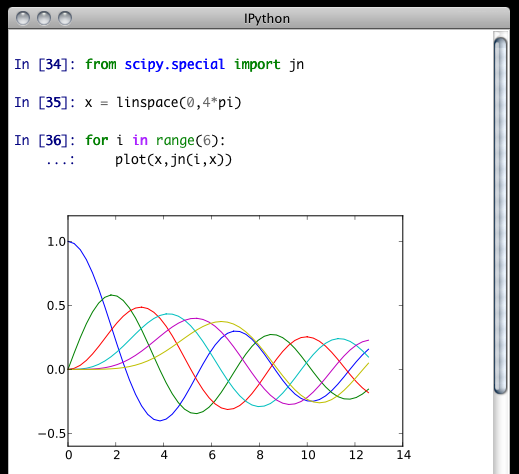
\includegraphics[width=0.6\linewidth]{besselj}}
    \caption{Cнимок экрана графической оболочки \textit{ipython} с встроенным графиком.}
    \label{img:besselj}
\end{figure}

\subsection{Конвейер обработки данных в системе Orange}
\label{orange-pipeline}

На рисунке \ref{img:series30} изображён конвейер статистической обработки данных в системе \textit{Orange}. Здесь он приведён целиком, в уменьшенном виде, для понимания общего расположения компонентов.

Конвейер имеет такой вид для всех трёх серий экспериментов. Далее мы рассмотрим части конвейера по отдельности и опишем каждый компонент, используемый в схеме анализа данных, изображённой на указанном выше рисунке.

\begin{figure}[H]
    \center{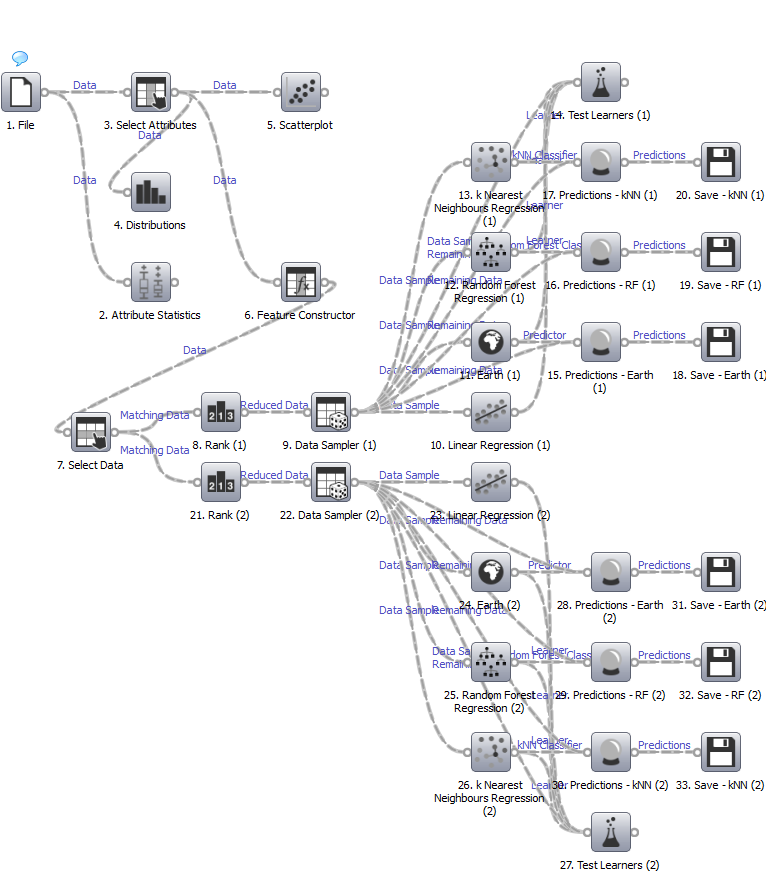
\includegraphics[scale=0.375]{series30}}
    \caption{Конвейер обработки данных в системе \textit{Orange}.}
    \label{img:series30}
\end{figure}

Первая часть конвейера "--- предварительная обработка данных перед построением модели. Она изображена на рисунке~\ref{img:series30-1}.

\begin{figure}[H]
    \center{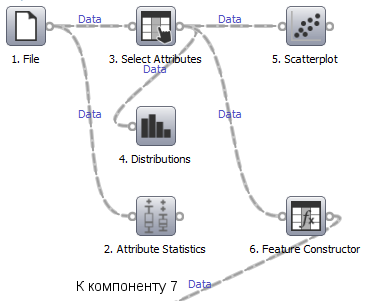
\includegraphics[scale=1]{series30-1}}
    \caption{Конвейер обработки данных в системе \textit{Orange}. Часть 1 "--- предварительная обработка.}
    \label{img:series30-1}
\end{figure}

Обработка данных в системе начинается с чтения входных данных в формате \textit{CSV} из файла "--- за это отвечает компонент \texttt{1.\,File}, находящийся в левом верхнем углу схемы. Отчёт по этому компоненту представлен на рисунке \ref{img:1-File}. Опишем формат входного файла.

\begin{figure}[H]
    \center{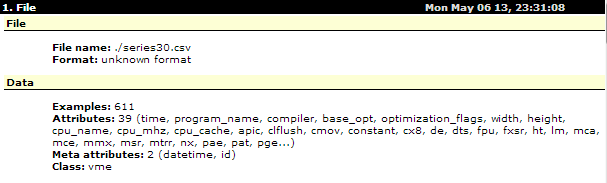
\includegraphics[scale=0.75]{1-File}}
    \caption{Компонент \texttt{1.\,File}. Входные данные в файле \textit{CSV}.}
    \label{img:1-File}
\end{figure}

Входной файл содержит таблицу, в которой столбцы "--- это названия свойств эксперимента, полученных во время его выполнения в инструментарии, а строки "--- собственно значения этих свойств. Приведём отрывок файла для пояснения его структуры (рисунок \ref{img:series.csv}). Многоточия означают опущенные части файла "--- поскольку число свойств достигает сорока, представить файл полностью не представляется возможным ввиду ограниченной ширины страницы. Свойство \texttt{id} также представлено в сокращённом виде "--- символы \texttt{..} означают опущенные части строки.

\Rotatebox{90}{
    \begin{minipage}{1.5\linewidth}
        \begin{figure}[H]
            \fontsize{10}{12}
            \begin{verbatim}
            id  datetime    time    program_name    compiler    base_opt    optimization_flags  width   height  cpu_name    cpu_mhz cpu_cache   apic ... vme
            5104..bd16    2013-04-17 22:25:29 0.0041661978    symm    gcc -O2 None    64  64  Intel(R) Xeon(R) CPU... 2666.76 6144    False ...    False
            5104..cc6d    2013-04-17 22:25:14 1.3440570831    symm    gcc -O2 None    256 256 Intel(R) Xeon(R) CPU... 2666.76 6144    False ...    False
            5104..d50b    2013-04-17 22:24:57 0.121064496 symm    gcc -O2 None    128 128 Intel(R) Xeon(R) CPU... 2666.76 6144    False ...    False
            \end{verbatim}
            \caption{Отрывок входного файла.}
            \label{img:series.csv}
        \end{figure}
    \end{minipage}
}

Итак, первая строка файла -- названия свойств. \texttt{id} "--- уникальный идентификатор эксперимента, \texttt{datetime} "--- время его проведения в GMT, \texttt{time} "--- время исполнения программы, \texttt{program_name} "--- название программы, \texttt{compiler} "--- название используемого компилятора, \texttt{base_opt} "--- базовый уровень оптимизации программы компилятором, \texttt{optimization_flags} "--- дополнительные настройки оптимизации, \texttt{width} "--- число столбцов в обрабатываемой матрице, \texttt{height} "--- число строк в обрабатываемой матрице, \texttt{cpu_name} "--- название процессора, на котором исполнялась программа, \texttt{cpu_mhz} "--- частота процессора, \texttt{cpu_cache} "--- объём кэша третьего уровня. Все остальные свойства, начиная с \texttt{apic} и заканчивая \texttt{vme} "--- двоичные свойства наличия у процессора поддержки определённой возможности, такой как, например, набора инструкций \textit{SSE}.

Отметим, что пунктирные линии на схеме обозначают передачу данных из одного компонента обработки данных в другой. Схема представляет собой дерево с корнем в узле \texttt{1.\,File}, причём данные передаются от корня к листьям. Таким образом, из узлов, которые не имеют дочерних, информация дальше не передаётся. Если у узла несколько дочерних узлов, данные передаются от родителя каждому ребёнку данного узла.

Компонент \texttt{2.\,Attribute~Statistics} используется для сбора и показа статистических показателей различных признаков экспериментов, содержащихся в наборе данных -- например, таких, как среднее и медианное значение признака. Выводимые им изображения можно найти в Приложении.

Компонент \texttt{3.\,Select~Attributes} (рисунок \ref{img:3-Select-Attributes}) применяется с целью установления структуры набора данных "--- в нём определяется, какие свойства экспериментов являются исходными данными для моделирования (признаками), а какие "--- выходными данными (предсказанными значениями). В данном случае все свойства экспериментов, кроме свойства \texttt{time} (время исполнения программы), являются признаками. Свойство \texttt{time} предсказывается моделью.

\begin{figure}[H]
    \center{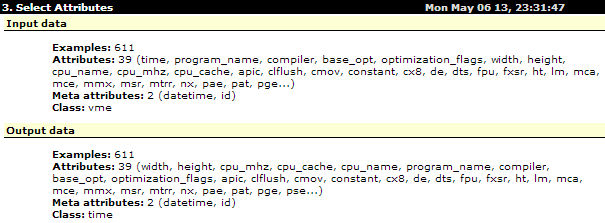
\includegraphics[scale=0.75]{3-Select-Attributes}}
    \caption{Компонент \texttt{3.\,Select~Attributes}. Определение структуры входных данных.}
    \label{img:3-Select-Attributes}
\end{figure}

Компонент \texttt{4.\,Distributions} отображает распределения различных атрибутов набора данных. Эти графики можно найти в Приложении.

Компонент \texttt{5.\,Scatterplot} строит точечные графики зависимости времени исполнения программы от других свойств эксперимента. Пример такого графика можно найти в Приложении. На нём завершается предварительный анализ входных данных.

Компонент \texttt{6.\,Feature Constructor} используется для создания дополнительного свойства эксперимента из уже присутствующих в наборе данных "--- свойства \texttt{size}, определяемого как $size = height \cdot width$ и имеющего смысл агрегированного размера обрабатываемой программой \texttt{symm} матрицы.

Компонент \texttt{7.\,Select~Data} (рисунок \ref{img:7-Select-Data}) может использоваться для фильтрации данных по различным признакам. Например, он может быть использован для удаления из набора данных всех экспериментов, для которых измеренное время исполнения оказалось менее 0,001 с вследствие артефактов измерения. Такая фильтрация может увеличить качество предсказания, поскольку результаты, которые очевидно являются шумом, удаляются из набора данных. Однако, в конечных версиях рассмотренных моделей данный компонент не был задействован, поскольку он требует тонкой настройки и снижает степень автоматизации моделирования.

\begin{figure}[H]
    \center{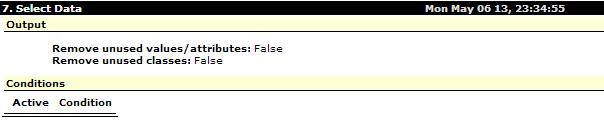
\includegraphics[scale=0.75]{7-Select-Data}}
    \caption{Компонент \texttt{7.\,Select~Data}. Выбор данных из набора.}
    \label{img:7-Select-Data}
\end{figure}

На этом предварительная обработка данных завершается и начинается собственно построение модели. Компоненты под номерами с 8 по 20 и с 20 по 33 полностью аналогичны. Они представляют собой две ветви конвейера, в одной из которых (с компонентами 8--20) используется простейшая модель на основе единственного признака, а в другой (с компонентами 20--33) "--- более сложная модель на основе четырёх или пяти признаков.

Опишем обе ветви конвейера, начиная с части, отвечающей за ранжирование признаков и выборку объектов. Эта часть схемы изображена на рисунке~\ref{img:series30-2}.

\begin{figure}[H]
    \center{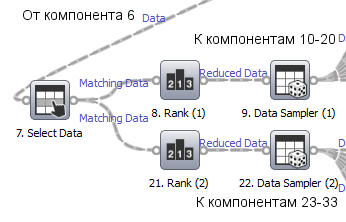
\includegraphics[scale=1]{series30-2}}
    \caption{Конвейер обработки данных в системе \textit{Orange}. Часть 2 "--- ранжирование признаков и выборка объектов.}
    \label{img:series30-2}
\end{figure}

Компонент \texttt{8.\,Rank~(1)} (рисунок \ref{img:8-Rank-1}) и его аналог \texttt{21.\,Rank~(2)}  выбирает $S$ наиболее значимых признаков набора данных, при этом $S = 1$ для компонента 8 и $S = 4$ или $S = 5$ для компонента 21. Выбор $S = 4$ или $S = 5$ зависит от результата работы алгоритма выделения важных признаков и для первой серии экспериментов $S = 4$, а для второй и третьей "--- $S = 5$. Согласно рассуждениям, приведённым ниже в разделе~\ref{choice-of-feature-ranking-algorithm}, в качестве алгоритма ранжирования признаков во всех случаях используется алгоритм \textit{Earth}.

\begin{figure}[H]
    \center{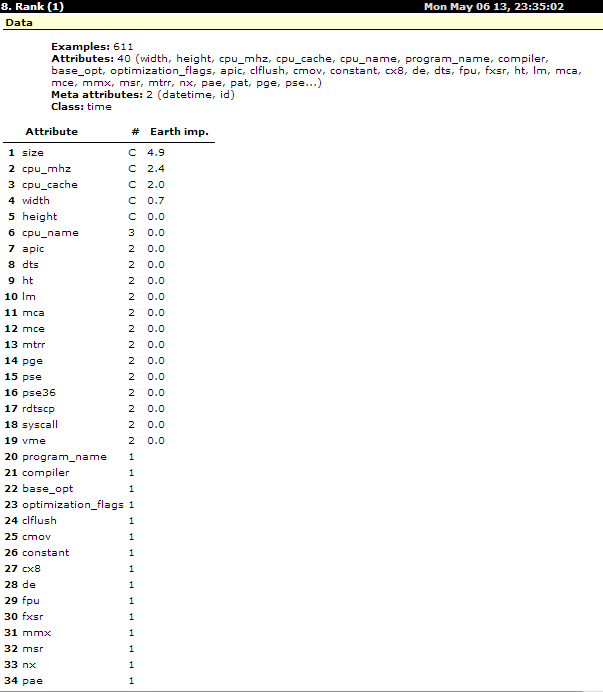
\includegraphics[scale=0.75]{8-Rank-1}}
    \caption{Компонент \texttt{8.\,Rank~(1)}. Выбор признаков.}
    \label{img:8-Rank-1}
\end{figure}

Остановимся подробнее на выборе алгоритма ранжирования признаков.

\paragraph{Алгоритм ранжирования признаков.}
\label{choice-of-feature-ranking-algorithm}

В системе статистической обработки данных Orange доступны следующие алгоритмы ранжирования признаков модели: \textit{Relief~F, MSE, Earth Importance} и \textit{Random Forest Importance}. В ходе изучения третьей серии экспериментов были получены результаты ранжирования признаков, показанные на рисунке~\ref{img:ranking-full}.

\begin{figure}[H]
    \center{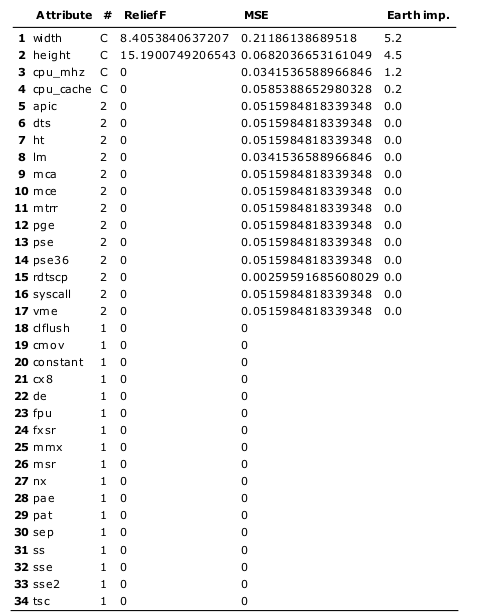
\includegraphics[scale=0.75]{ranking-full}}
    \caption{Сравнение алгоритмов ранжирования признаков модели.}
    \label{img:ranking-full}
\end{figure}

Как можно видеть, алгоритм \textit{Relief~F} показал результаты, целиком отбрасывающие влияние свойств \texttt{cpu_mhz} и \texttt{cpu_cache}, а также всех остальных особенностей аппаратной платформы. Это заведомо неверно, поскольку известно, что характеристики аппаратного обеспечения влияют на производительность программы. Этот алгоритм выделил только два самых очевидных свойства, оказывающих влияние на производительность.

Алгоритм \textit{MSE} также присвоил наибольшие веса свойствам \texttt{width} и \texttt{height}, а на третье место по важности поставил \texttt{cpu_cache}, что выглядит разумно. Однако, данный алгоритм присвоил одинаковые веса многим признакам, которые просто коррелируют с изменением свойств \texttt{cpu_mhz} и \texttt{cpu_cache}, но не обнаружил корреляции -- таким образом, свойства \texttt{apic, dts} и другие получили вес $0,05159...$. При этом истинно важный признак \texttt{cpu_mhz} был оценён важностью, меньшей чем у всех этих коррелирующих признаков, что свидетельствует о невозможности применения этого алгоритма для нашей задачи.

Алгоритм \textit{Earth Importance} выявил все четыре признака, которые являются важными в нашей модели -- число строк и столбцов в обрабатываемой матрице, частоту используемого процессора и объём его кэша. При этом <<паразитные>> коррелирующие признаки не были оценены алгоритмом как важные "--- таким образом мы избавляемся от лишних свойств в модели и делаем её минимально необходимой для адекватного описания предметной области.

Алгоритм \textit{Random Forest Importance} отработал на нашем наборе данных некорректно, вызвав программную ошибку в системе Orange. Он был исключён из дальнейшего рассмотрения.

Таким образом, мы выбираем \textit{Earth Importance} в качестве алгоритма ранжирования признаков.

Теперь продолжим рассмотрение конвейера обработки данных в системе \textit{Orange}.

Компоненты \texttt{9.\,Data~Sampler~(1)} и \texttt{22.\,Data~Sampler~(2)} производят случайный отбор 70\% данных из набора в учебный набор, а остальных 30\% "--- в проверочный набор данных. Это необходимо для проведения перекрёстной проверки, которая в данном случае является одно-проходной ввиду ограниченных ресурсов времени и невысокой степени автоматизации осуществления перекрёстной проверки в системе \textit{Orange}. При этом компонент 9 работает с моделью, построенной на основе единственного признака, который был оценён, как наиболее важный, компонентом 8. Компонент 22 работает с моделью на основе четырёх или пяти признаков, наиболее важных по результатам работы компонента 21. Далее мы не будем останавливаться на различиях моделей в ветвях (8--20) и (20--33).

\begin{figure}[H]
    \center{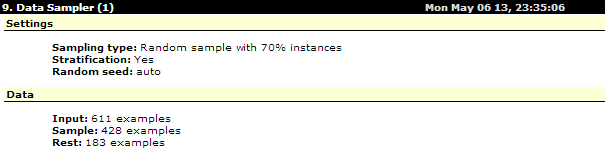
\includegraphics[scale=0.75]{9-Data-Sampler-1}}
    \caption{Компонент \texttt{9.\,Data~Sampler~(1)}. Отбор объектов в обучающую и проверочную выборки.}
    \label{img:9-Data-Sampler-1}
\end{figure}

На этом вторая часть схемы заканчивается и мы переходим собственно к обучению предсказателей для двух моделей "--- простейшей (с одним признаком) и более сложной (с четырьмя или пятью признаками).

На рисунках~\ref{img:series30-3}~и~\ref{img:series30-4} представлены две последние части конвейера обработки данных в \textit{Orange}. Они полностью аналогичны и отличаются тем, что первая (описывающая компоненты~10--20) получает данные от компонента~9, а вторая (компоненты~23--33) "--- от компонента~22. Это данные, включающие в себя один признак эксперимента и несколько (четыре или пять) признаков эксперимента, соответственно.

\begin{figure}[H]
    \center{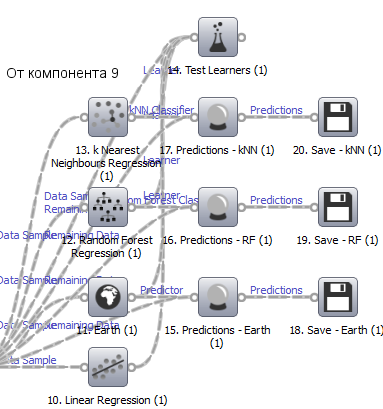
\includegraphics[scale=1]{series30-3}}
    \caption{Конвейер обработки данных в системе \textit{Orange}. Часть 3 "--- построение простейшей модели.}
    \label{img:series30-3}
\end{figure}

Компоненты \texttt{10.\,Linear~Regression~(1)} и \texttt{23.\,Linear~Regression~(2)} строят модели линейной регрессии на основе экспериментальных данных. Эти модели являются образцовыми. Это значит, что качество результатов данных моделей является нижней границей для качества результатов любых других моделей. Поскольку линейная регрессия является простейшим предсказателем, рассмотрение моделей, которые дают результаты хуже, чем линейная регрессия, не имеет смысла. Модели из компонентов 10 и 23 передаются в компоненты 14 и 27 соответственно, где те сравниваются с другими предсказателями по нескольким метрикам (см. ниже).

\begin{figure}[H]
    \center{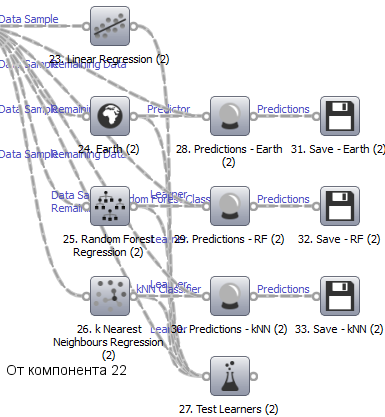
\includegraphics[scale=1]{series30-4}}
    \caption{Конвейер обработки данных в системе \textit{Orange}. Часть 3 "--- построение более сложной модели.}
    \label{img:series30-4}
\end{figure}

Компоненты \texttt{11.\,Earth~(1), 12.\,Random~Forest Regression~(1), 13.\,k~Nearest~Neighbours Regression~(1)} и \texttt{24.\,Earth~(2), 25.~Random~Forest Regression~(2), 26.\,k~Nearest~Neighbours Regression~(2)} являются модулями построения предсказателей \textit{Earth, Random~Forest} и \textit{kNN} для ветвей (8--20) и (20--33) соответственно.

\begin{figure}[H]
    \center{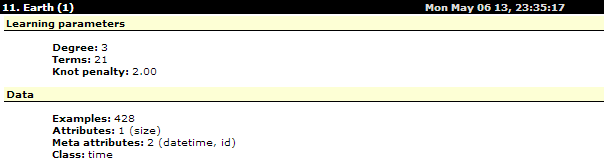
\includegraphics[scale=0.75]{11-Earth-1}}
    \caption{Компонент \texttt{11.\,Earth~(1)}. Предсказатель \textit{Earth} для модели с одним признаком.}
    \label{img:11-Earth-1}
\end{figure}

\begin{figure}[H]
    \center{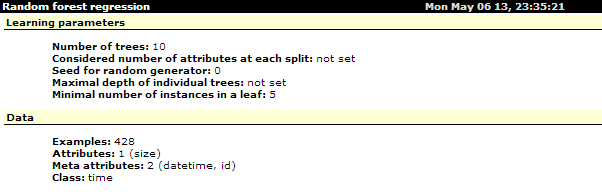
\includegraphics[scale=0.75]{12-RF-1}}
    \caption{Компонент \texttt{12.\,Random~Forest~(1)}. Предсказатель \textit{Random~Forest} для модели с одним признаком.}
    \label{img:12-RF-1}
\end{figure}

\begin{figure}[H]
    \center{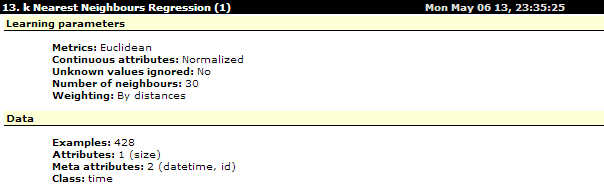
\includegraphics[scale=0.75]{13-kNN-1}}
    \caption{Компонент \texttt{13.\,kNN~(1)}. Предсказатель \textit{k~Nearest~Neighbours} для модели с одним признаком.}
    \label{img:13-kNN-1}
\end{figure}

\begin{figure}[H]
    \center{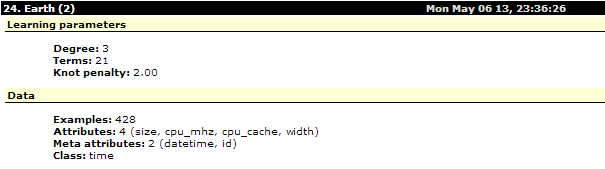
\includegraphics[scale=0.75]{24-Earth-2}}
    \caption{Компонент \texttt{24.\,Earth~(2)}. Предсказатель \textit{Earth} для модели с четырьмя признаками.}
    \label{img:24-Earth-2}
\end{figure}

\begin{figure}[H]
    \center{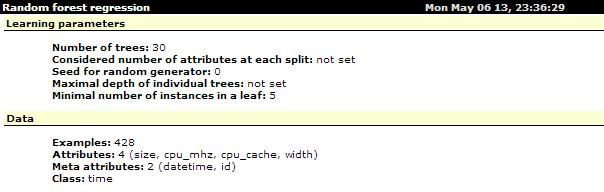
\includegraphics[scale=0.75]{25-RF-2}}
    \caption{Компонент \texttt{25.\,Random~Forest~(2)}. Предсказатель \textit{Random~Forest} для модели с четырьмя признаками.}
    \label{img:25-RF-2}
\end{figure}

\begin{figure}[H]
    \center{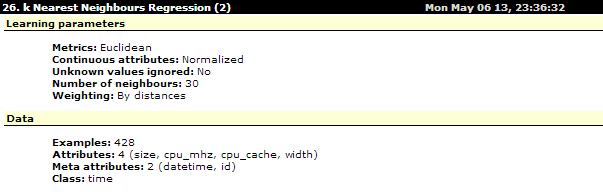
\includegraphics[scale=0.75]{26-kNN-2}}
    \caption{Компонент \texttt{26.\,kNN~(2)}. Предсказатель \textit{k~Nearest~Neighbours} для модели с четырьмя признаками.}
    \label{img:26-kNN-2}
\end{figure}

После обучения предсказателей их параметры передаются в компоненты сравнения качества результатов \texttt{14.\,Test~Learners~(1)} и \texttt{27.\,Test~Learners~(2)}. Кроме этого, они используются для построения предсказаний в компонентах \texttt{15.\,Predictions - Earth~(1), 16.\,Predictions - RF~(1), 17.\,Predictions - kNN~(1)} и {28.\,Predictions - Earth~(2), 29.\,Predictions - RF~(2), 30.\,Predictions - kNN~(2)} соответсвенно.

\begin{figure}[H]
    \center{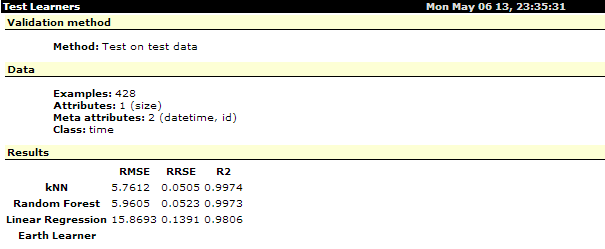
\includegraphics[scale=0.75]{14-Test-Learners-1}}
    \caption{Компонент \texttt{26.\,Test~Learners~(2)}. Сравнение предсказателей для модели с одним признаком.}
    \label{img:14-Test-Learners-1}
\end{figure}

\begin{figure}[H]
    \center{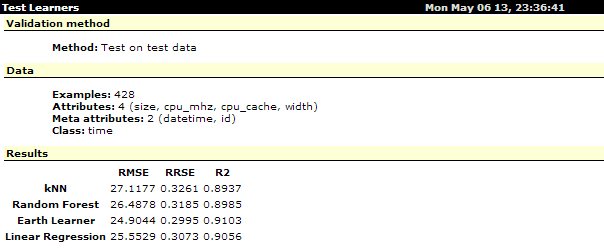
\includegraphics[scale=0.75]{27-Test-Learners-2}}
    \caption{Компонент \texttt{27.\,Test~Learners~(2)}. Сравнение предсказателей для модели с четырьмя признаками.}
    \label{img:27-Test-Learners-2}
\end{figure}

После построения предсказаний, они сохраняются в файлах \textit{CSV} с помощью компонентов \texttt{18.\,Save - Earth~(1), 19.\,Save - RF~(1), 20.\,Save - kNN~(1)} и \texttt{31.\,Save - Earth~(2), 32.\,Save - RF~(2), 33.\,Save - kNN~(2)} в формате, аналогичном формату исходного файла, загруженного компонентом \texttt{1.\,File}.

% Исследование эффективности
\section{Оценка эффективности}
В рамках оценки эффективности разработанного программного комплекса проведём несколько серий экспериментов с его помощью, а затем осуществим анализ экспериментальных данных.

Далее в этом разделе мы последовательно рассмотрим следующие серии экспериментов и их анализ:
\begin{itemize}
    \item серия экспериментов по проверке точности измерения времени;
    \item серия экспериментов по сравнению производительности программ, собранных компиляторами GCC и LLVM на настройках «по умолчанию»;
    \item группа серий экспериментов по моделированию и предсказанию производительности программы из набора Polybench на различном аппаратном обеспечении:
    \begin{itemize}
        \item серия экспериментов по моделированию и предсказанию производительности при размере входных данных, который меняется по степенному закону, а обе размерности входных данных одинаковы;
        \item серия экспериментов по моделированию и предсказанию производительности при размере входных данных, который меняется случайно при равномерном распределении случайной величины, а обе размерности входных данных одинаковы;
        \item серия экспериментов по моделированию и предсказанию производительности при размере входных данных, который меняется случайно при равномерном распределении случайной величины, а размерности входных данных не одинаковы.
    \end{itemize}
\end{itemize}

\subsection{Серия экспериментов по проверке точности измерения времени}
\label{series-accuracy}
Для проверки точности измерения времени проведём следующий эксперимент.

Сгенерируем семейство программ, которые не делают ничего, кроме вызова функции стандартной библиотеки \textit{C} \texttt{usleep}. Аргументами функции будет число $10^n$, где $n$ --- число от одного до шести включительно. Таким образом, после запуска программа устанавливает таймер на заданное число микросекунд (от 1 мкс до 1000000 мкс = 1 с), останавливается и после его срабатывания завершает работу.

Далее на рис. \ref{img:calibration} приведён график измеренного времени исполнения семейства таких программ и «реального» времени их выполнения --- т.е. времени, указанного в аргументе функции, создающей таймер. График построен с помощью инструментария в автоматическом режиме.

\begin{figure}[p]
    \center{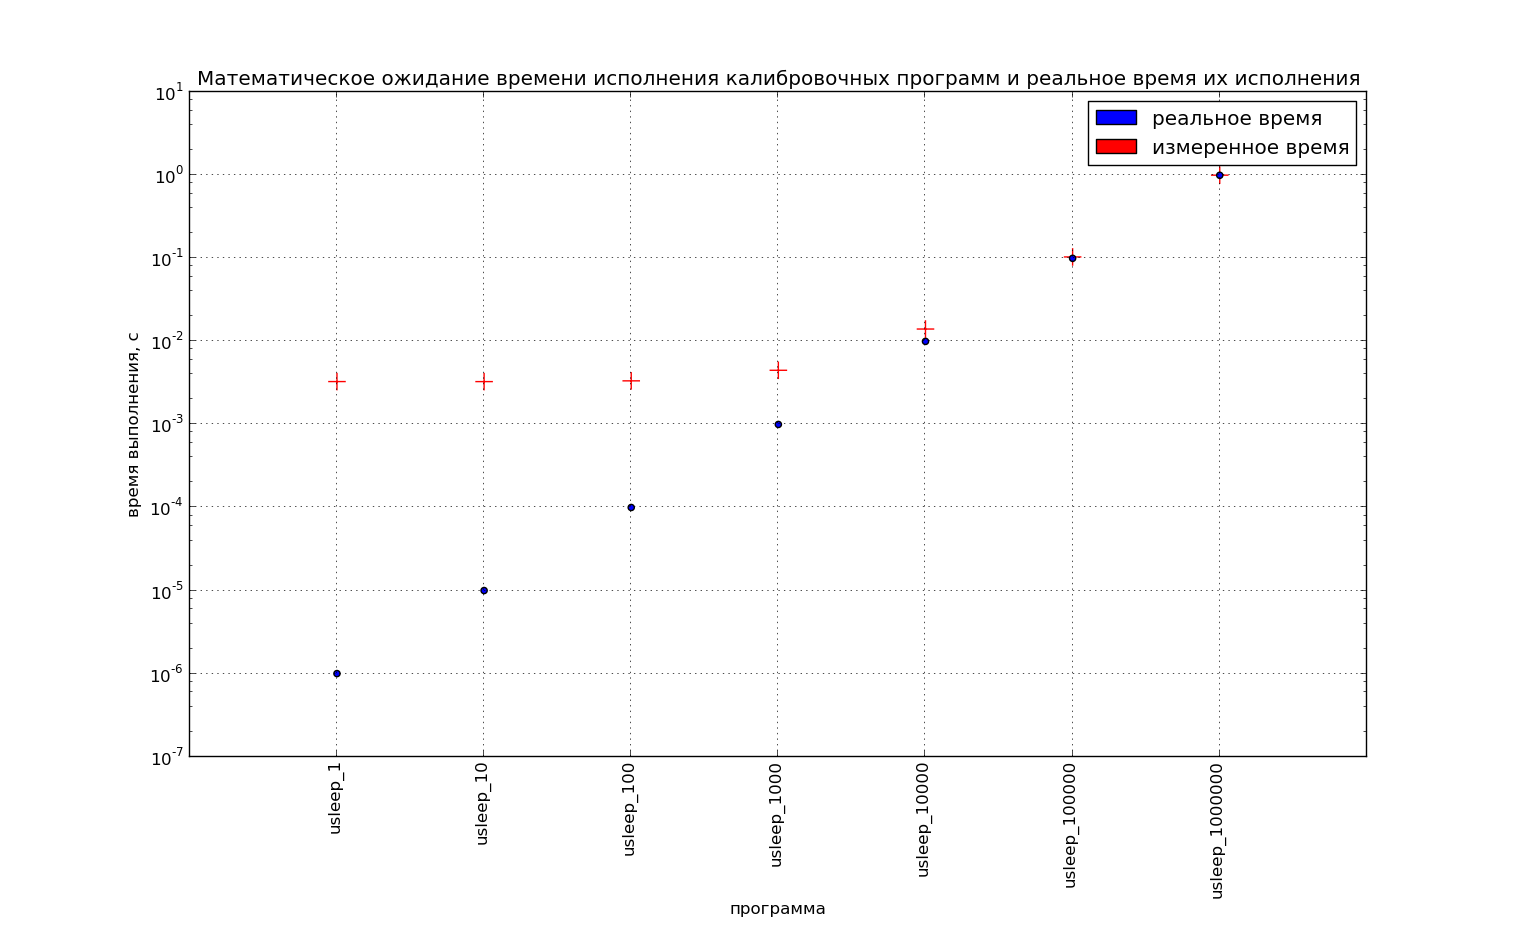
\includegraphics[width=1\linewidth]{calibration}}
    \caption{График измеренного и реального времени исполнения семейства калибровочных программ}
    \label{img:calibration}
\end{figure}

Как мы видим на рис. \ref{img:calibration}, измеренное время асимптотически приближается к значению между $10^{-2}$ и $10^{-3}$ --- около 0,005.

Из этого можно сделать вывод, что существуют постоянные расходы на запуск программы из нашей системы и их можно вычесть из измеренного времени для повышения точности измерения. Для этого мы вычисляем время выполнения пустой программы (согласно описанной в подразделе~\ref{sssect:calibration} методике), а затем вычитаем его из каждого измеренного результата выполнения реальных программ.

На рис. \ref{img:calibration-offset} показан график измеренного времени в данном эксперименте с учётом накладных расходов.

\begin{figure}[p]
    \center{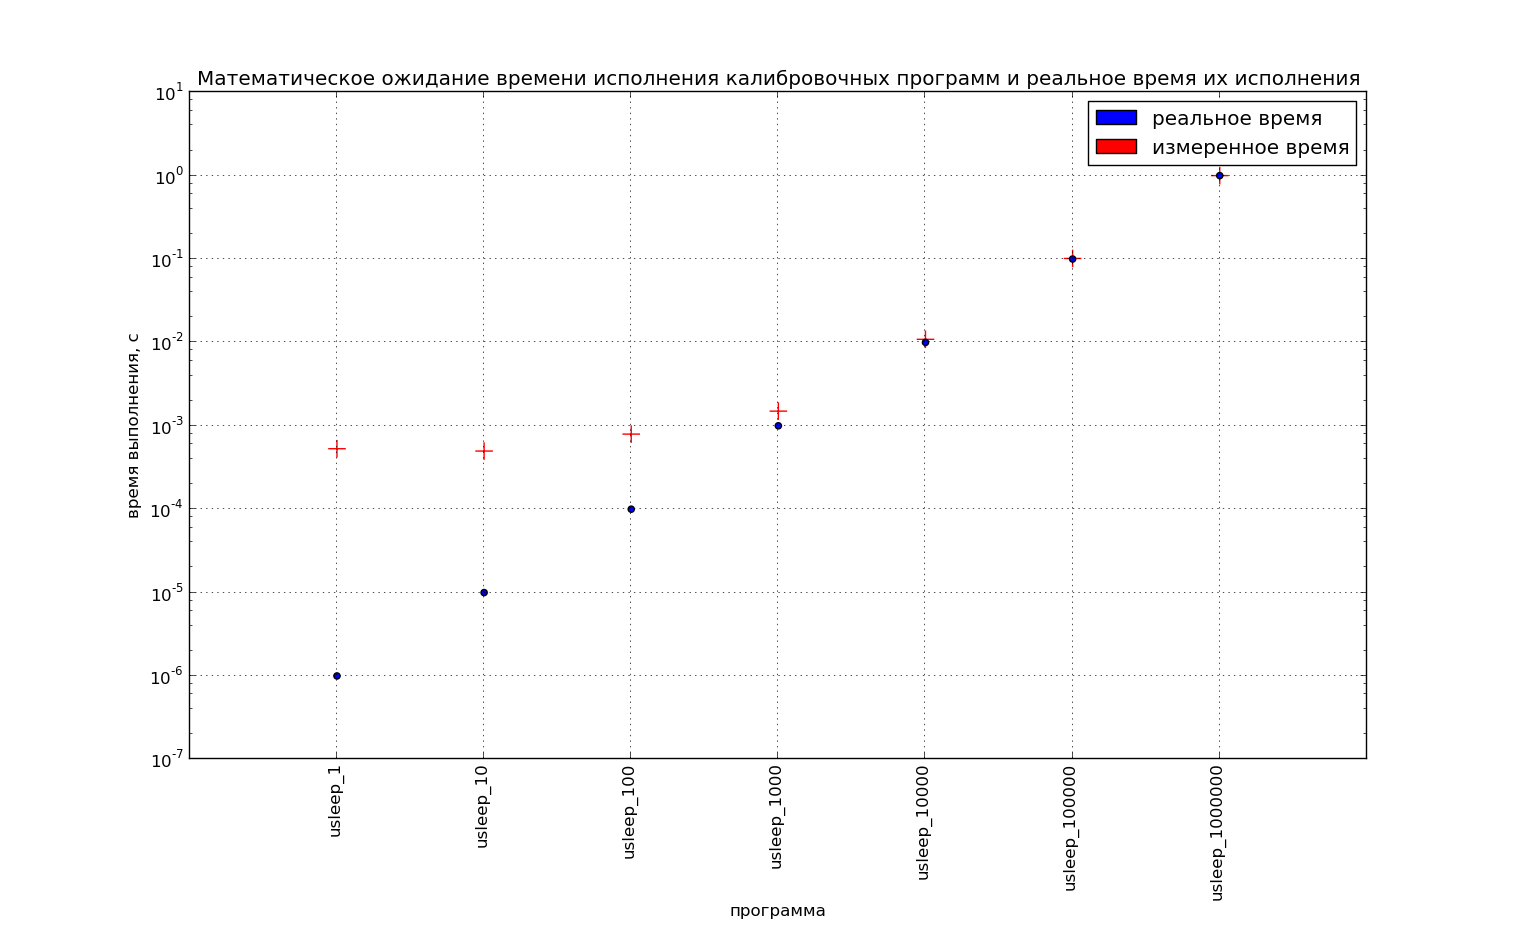
\includegraphics[width=1\linewidth]{calibration-offset}}
    \caption{График измеренного и реального времени исполнения семейства калибровочных программ с учётом накладных расходов}
    \label{img:calibration-offset}
\end{figure}

Далее на рис. \ref{img:default_calibration} приведён текстовый вывод из инструментария результата описанного эксперимента с учётом накладных расходов.

\begin{figure}[H]
    \fontsize{10}{12}
    \begin{verbatim}
        Experiment performed:
            Real time: 0.000001
            Measured time: 0.000531
            Relative error: 530.11
        
        Experiment performed:
            Real time: 0.000010
            Measured time: 0.000498
            Relative error: 48.79
        
        Experiment performed:
            Real time: 0.000100
            Measured time: 0.000795
            Relative error: 6.95
        
        Experiment performed:
            Real time: 0.001000
            Measured time: 0.001499
            Relative error: 0.50
        
        Experiment performed:
            Real time: 0.010000
            Measured time: 0.010893
            Relative error: 0.09
        
        Experiment performed:
            Real time: 0.100000
            Measured time: 0.101603
            Relative error: 0.02
        
        Experiment performed:
            Real time: 1.000000
            Measured time: 1.001015
            Relative error: 0.00
    \end{verbatim}
    \caption{Результат работы программы для описанного выше эксперимента.}
    \label{img:default_calibration}
\end{figure}

Таким образом, инструментарий позволяет производить достаточно точное измерение времени (ошибка в пределах 10\%) для программ, исполняющихся 10 мс и более.


\subsection{Серия экспериментов по сравнению компиляторов GCC и LLVM на тестовом наборе Polybench}
\label{series-llvm-vs-gcc}
На рис. \ref{img:gcc-vs-clang} сравнивается время исполнения программ, собранных компиляторами GCC и LLVM соответственно на уровне оптимизации '-O2'. Компилятор на этом уровне оптимизации в подавляющем большинстве случаев генерирует наиболее быстрый код (относительно уровней '-O0' и '-O1').

\begin{figure}[!bH]
    \center{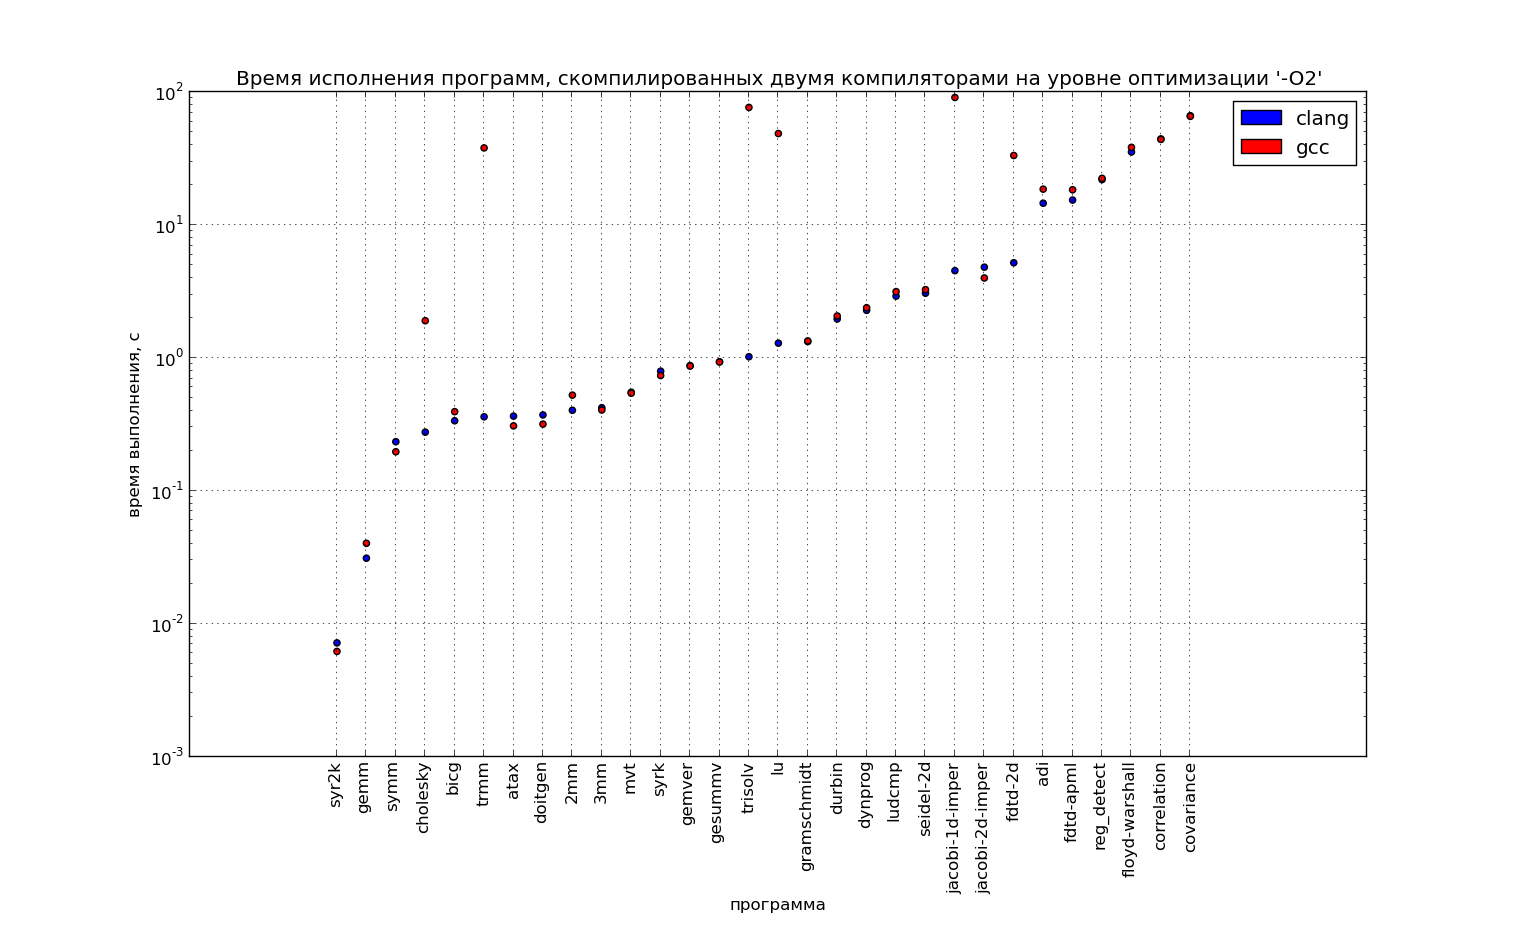
\includegraphics[width=1\linewidth]{gcc-vs-clang}}
    \caption{График времени исполнения программ из набора Polybench для двух компиляторов.}
    \label{img:gcc-vs-clang}
\end{figure}

Как мы видим из графика, на большинстве программ оба компилятора показывают примерно одинаковую производительность. Однако на шести программах компилятор LLVM серьёзно превосходит GCC -- это программы \textit{cholesky, trmm, trisolv, lu, jacobi-1d-imper, fdtd-2d}. Вероятно, LLVM использует лучший векторизатор кода, что оказывает большое влияние в этих специфических случаях. В целом, указанные программы относятся к различным классам -- это программы решения СЛАУ и СДУ. Выяснение конкретных причин этого превосходства выходит за рамки данной работы.

\subsection{Группа серий экспериментов по моделированию и предсказанию производительности программы из набора Polybench на различном аппаратном обеспечении}

Одной из возможностей, предоставляемых инструментарием, является статистический анализ данных серии экспериментов с целью предсказания производительности программ на различном аппаратном обеспечении при различном размере и форме входных данных.

Для этого выберем программу из набора Polybench, которую будем анализировать. Критериями выбора являются факторы, приведённые ниже.
\begin{itemize}
    \item Время исполнения программы при различных размерах и формах входных данных должно быть не слишком велико. Поскольку в рамках серии экспериментов программа должна быть исполнена статистически значимое число раз (по крайней мере 100), мы должны выбрать программу с учётом доступных ресурсов машинного времени и общих ресурсов времени, которое можно потратить на исследование.
    \item Время исполнения программы при различных размерах и формах входных данных должно быть не слишком мало. При уменьшении времени однократного исполнения программы погрешность измерения реального времени исполнения возрастает -- до 50\% при времени однократного исполнения 0,001 с (см. раздел \ref{series-accuracy}). Поэтому мы должны выбрать программу, которая исполняется секунду или более, для достижения оптимальных результатов. При указанном времени исполнения точность измерения времени достигает как минимум 99\% (раздел \ref{series-accuracy}).
\end{itemize}

На основании указанных критериев и данных, полученных в рамках серии экспериментов, описанной в разделе \ref{series-llvm-vs-gcc}, выбираем программу \texttt{symm} в качестве анализируемой.

Мы осуществим три серии экспериментов по моделированию и предсказанию производительности программы \texttt{symm} из набора Polybench. Они перечислены ниже.
\begin{enumerate}
    \item Первая серия экспериментов характеризуется размерами входных данных $M$ (число столбцов обрабатываемой матрицы) и $N$ (число строк обрабатываемой матрицы), задаваемыми по степенному закону $M = N = 2^x, x = [1;12]$. Таким образом, $M = N \in [2;4096]$.
    \item Вторая серия экспериментов характеризуется размерами входных данных $M$ и $N$, задаваемыми случайно из диапазона [2;2048]: $M = N = rand([2;2048])$, где $rand$ -- функция случайного выбора целого числа из указанного диапазона по равномерному закону распределения. Таким образом, $M = N \in [2;2048]$.
    \item Третья серия экспериментов характеризуется размерами входных данных $M$ и $N$, задаваемыми случайно и независимо из диапазона [2;2048]: $M = rand_1([2;2048]), N = rand_2([2;2048])$, где $rand_i, i \in [1;2]$ -- выборки случайного выбора целого числа из указанного диапазона по равномерному закону распределения (в данном случае выбираются два случайных числа). Таким образом, $M, N \in [2;2048]$.
\end{enumerate}

В каждой серии экспериментов производится обучение трёх предсказателей -- \textit{Earth, Random Forest и k-Nearest Neigbour} -- и последующее предсказание производительности программы \texttt{symm} на различных аппаратных платформах и при различных размерах входных данных. Обучение производится на двух различных моделях -- простейшей (включающей всего один признак из набора экспериментальных данных), и более сложной (включающей в себя до пяти признаков из набора экспериментальных данных). Обучение и предсказание на основе экспериментальных данных производится в системе статистической обработки данных с открытым исходным кодом Orange \cite{orange}.

Опишем систему моделирования и предсказания более подробно. Она организована в форме конвейера с ветвлениями. Более подробно система описана в следующем разделе.

\subsubsection{Конвейер статистической обработки данных в системе Orange}
На рисунке \ref{img:series30} изображён конвейер статистической обработки данных в системе Orange. Он имеет такой вид для всех трёх серий экспериментов. Далее мы опишем каждый компонент, используемый в схеме анализа данных, изображённой на указанном рисунке.

\begin{figure}[H]
    \center{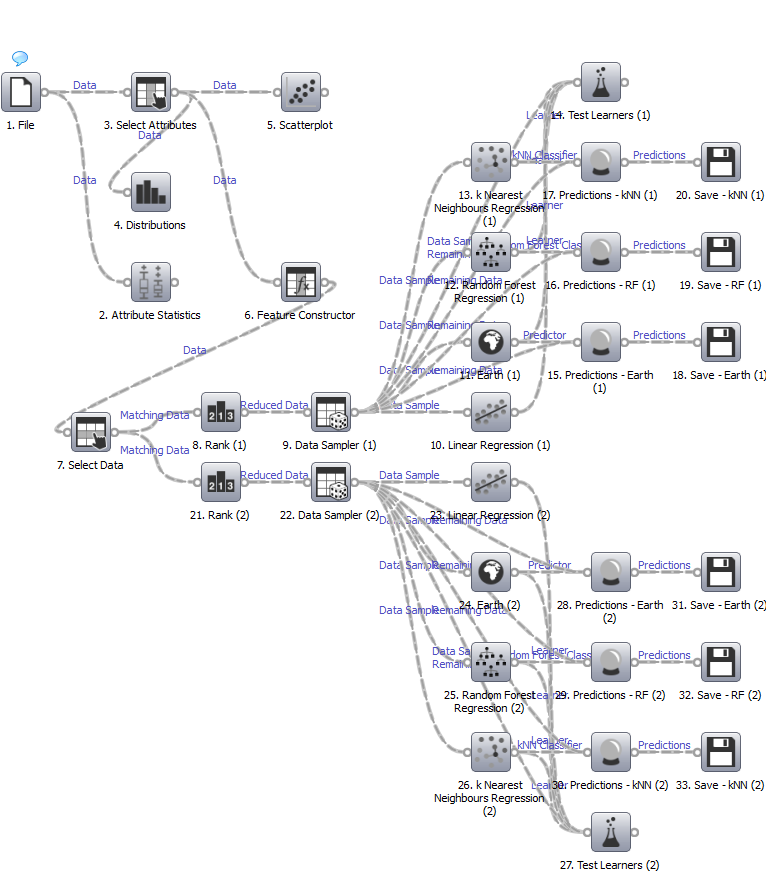
\includegraphics[width=1\linewidth]{series30}}
    \caption{Конвейер обработки данных в системе Orange.}
    \label{img:series30}
\end{figure}

Обработка данных в системе начинается с чтения входных данных в формате CSV из файла -- за это отвечает компонент \texttt{1. File}, находящийся в левом верхнем углу схемы. Опишем формат входного файла.

Входной файл содержит таблицу, в которой столбцы -- это названия свойств эксперимента, полученных во время его выполнения в инструментарии, а строки -- собственно значения этих свойств. Приведём отрывок файла для пояснения его структуры (рисунок \ref{img:series.csv}). Многоточия означают опущенные части файла -- поскольку число свойств достигает сорока, представить файл полностью не представляется возможным ввиду ограниченной ширины страницы. Свойство \texttt{id} также представлено в сокращённом виде -- символы \texttt{..} означают опущенные части строки.

\Rotatebox{90}{
    \begin{minipage}{1.5\linewidth}
        \begin{figure}[H]
            \fontsize{10}{12}
            \begin{verbatim}
id  datetime    time    program_name    compiler    base_opt    optimization_flags  width   height  cpu_name    cpu_mhz cpu_cache   apic ... vme
5104..bd16    2013-04-17 22:25:29 0.0041661978    symm    gcc -O2 None    64  64  Intel(R) Xeon(R) CPU... 2666.76 6144    False ...    False
5104..cc6d    2013-04-17 22:25:14 1.3440570831    symm    gcc -O2 None    256 256 Intel(R) Xeon(R) CPU... 2666.76 6144    False ...    False
5104..d50b    2013-04-17 22:24:57 0.121064496 symm    gcc -O2 None    128 128 Intel(R) Xeon(R) CPU... 2666.76 6144    False ...    False
            \end{verbatim}
            \caption{Отрывок входного файла.}
            \label{img:series.csv}
        \end{figure}
    \end{minipage}
}

Итак, первая строка файла -- названия свойств. \texttt{id} -- уникальный идентификатор эксперимента, \texttt{datetime} -- время его проведения в GMT, \texttt{time} -- время исполнения программы, \texttt{program_name} -- название программы, \texttt{compiler} -- название используемого компилятора, \texttt{base_opt} -- базовый уровень оптимизации программы компилятором, \texttt{optimization_flags} -- дополнительные настройки оптимизации, \texttt{width} -- число столбцов в обрабатываемой матрице, \texttt{height} -- число строк в обрабатываемой матрице, \texttt{cpu_name} -- название процессора, на котором исполнялась программа, \texttt{cpu_mhz} -- частота процессора, \texttt{cpu_cache} -- размер кэша третьего уровня. Все остальные свойства, начиная с \texttt{apic} и заканчивая \texttt{vme} -- двоичные свойства наличия у процессора поддержки определённой возможности, такой как, например, набора инструкций SSE.

Отметим, что пунктирные линии на схеме обозначают передачу данных из одного компонента обработки данных в другой. Схема представляет собой дерево с корнем в узле \texttt{1. File}, причём данные передаются от корня к листьям. Таким образом, из узлов, которые не имеют дочерних, информация дальше не передаётся. Если у узла несколько дочерних узлов, данные передаются от родителя каждому ребёнку данного узла.

Компонент \texttt{2. Attribute Statistics} используется для сбора и показа статистических показателей различных признаков экспериментов, содержащихся в наборе данных -- например, таких, как среднее и медианное значение признака. Компонент \texttt{3. Select Attributes} применяется с целью установления структуры набора данных -- в нём определяется, какие свойства экспериментов являются исходными данными для моделирования (признаками), а какие -- выходными данными (предсказанными значениями). В данном случае все свойства экспериментов, кроме свойства \texttt{time} (время исполнения программы), являются признаками. Свойство \texttt{time} предсказывается моделью. Компонент \texttt{4. Distributions} отображает распределения различных атрибутов набора данных. Компонент \texttt{5. Scatterplot} строит точечные графики зависимости времени исполнения программы от других свойств эксперимента. На нём завершается предварительный анализ входных данных.

Компонент \texttt{6. Feature Constructor} используется для создания дополнительного свойства эксперимента из уже присутствующих в наборе данных -- свойства \texttt{size}, определяемого как $size = height \cdot width$ и имеющего смысл агрегированного размера обрабатываемой программой \texttt{symm} матрицы.

Компонент \texttt{7. Select Data} может использоваться для фильтрации данных по различным признакам. Например, он может быть использован для удаления из набора данных всех экспериментов, для которых измеренное время исполнения оказалось менее 0,001 с вследствие артефактов измерения. Такая фильтрация может увеличить качество предсказания, поскольку результаты, которые очевидно являются шумом, удаляются из набора данных. Однако, в конечных версиях рассмотренных моделей данный компонент не был задействован, поскольку он требует тонкой настройки и снижает степень автоматизации моделирования.

На этом предварительная обработка данных завершается и начинается собственно построение модели. Компоненты под номерами с 8 по 20 и с 20 по 33 полностью аналогичны. Они представляют собой две ветви конвейера, в одной из которых (с компонентами 8-20) используется простейшая модель на основе единственного признака, а в другой (с компонентами 20-33) -- более сложная модель на основе четырёх или пяти признаков.

Опишем обе ветви конвейера.

Компонент \texttt{8. Rank (1)} и его аналог \texttt{21. Rank (2)} выбирает $S$ наиболее значимых признаков набора данных, при этом $S = 1$ для компонента 8 и $S = 4$ или $S = 5$ для компонента 21. Выбор $S = 4$ или $S = 5$ зависит от результата работы алгоритма выделения важных признаков и для первой и второй серий экспериментов $S = 4$, а для третьей -- $S = 5$.

Компоненты \texttt{9. Data Sampler (1)} и \texttt{22. Data Sampler (2)} производят случайный отбор 70\% данных из набора в учебный набор, а остальных 30\% -- в проверочный набор данных. Это необходимо для проведения перекрёстной проверки, которая в данном случае является одно-проходной ввиду ограниченных ресурсов времени и невысокой степени автоматизации осуществления перекрёстной проверки в системе Orange. При этом компонент 9 работает с моделью, построенной на основе единственного признака, который был оценён, как наиболее важный, компонентом 8. Компонент 22 работает с моделью на основе четырёх или пяти признаков, наиболее важных по результатам работы компонента 21. Далее мы не будем останавливаться на различиях моделей в ветках (8-20) и (20-33).

Компоненты \texttt{10. Linear Regression (1)} и \texttt{23. Linear Regression (2)} строят модели линейной регрессии на основе экспериментальных данных. Эти модели являются образцовыми. Это значит, что качество результатов данных моделей является нижней границей для качества результатов любых других моделей. Поскольку линейная регрессия является простейшим предсказателем, рассмотрение моделей, которые дают результаты хуже, чем линейная регрессия, не имеет смысла. Модели из компонентов 10 и 23 передаются в компоненты 14 и 27 соответственно, где те сравниваются с другими предсказателями по нескольким метрикам (см. ниже).

Компоненты \texttt{11. Earth (1), 12. Random Forest Regression (1), 13. k Nearest Neighbours Regression (1)} и \texttt{11. Earth (2), 12. Random Forest Regression (2), 13. k Nearest Neighbours Regression (2)} являются модулями построения предсказателей Earth, Random Forest и kNN для ветвей (8-20) и (20-33) соответственно.

Рассмотрим результаты выполнения этих серий экспериментов и моделирования производительности программы \texttt{symm} в каждом случае.

\subsubsection{Серия экспериментов №1}

\pagebreak
% Экономика
\section{Экономически-организационная часть}
\subsection{Введение}
Экономическая часть посвящена разработке комплекса мероприятий организационно–экономического и финансового планов, которые необходимо выполнить для создания программного продукта, позволяющего проводить анализ и моделирование производительности программ.

Система разработана на языке программирования Python, и включает в себя группу проектов анализа данных в системе проведения статистических исследований Orange. Программный продукт не может быть интегрирован в другие программные комплексы и предназначен для внутреннего использования. Заказчиком является структурное подразделение МГТУ им. Н. Э. Баумана.
Данный проект не преследует цель получения прибыли.

\subsection{Основные этапы проекта разработки нового изделия}
Основные этапы проекта разработки нового изделия представлены в таблице \ref{tab:development-stages}.

\begin{table}[H]
    \caption{\label{tab:development-stages}Основные этапы разработки проекта}
    \begin{tabular}[H]{|l|p{5cm}|p{8cm}|}
        \hline
        № & Условное обозначение & Описание\\
        \hline
        1 & Техническое задание (ТЗ) & Предпроектное обследование. Постановка задачи по созданию программного продукта\\
        \hline
        2 & Эскизный проект (ЭП) & Проработка использования основных технологий и инструментов, необходимых для выполнения программного продукта\\
        \hline
        3 & Технорабочий проект (ТП) & Разработка модели анализа: структуры данных и реализации алгоритмов анализа. Разработка программного решения\\
        \hline
        4 & Документация и внедрение (В) & Подготовка и передача программного продукта и программной документации\\
        \hline
    \end{tabular}
\end{table}

% Охрана труда и экология
\section{Охрана труда и экология}
\subsection{Проектирование рабочего места оператора ПЭВМ}
Требования к компьютерной технике и к условиям работы с ней в Российской Федерации регламентируются санитарными нормами и правилами СанПиН 2.2.2/2.4.1340-03 и СанПиН 2.2.2.000-02. Рассмотрим основные нормы, необходимые для проектирования рабочего места оператора ПЭВМ.
\subsubsection{Требования к рабочим помещениям}
Согласно СанПиН 2.2.2/2.4.1340-03, помещения для работы с компьютерами должны оборудоваться системами отопления, кондиционирования воздуха или эффективной приточно-вытяжной вентиляцией. Звукоизоляция помещений и звукопоглощение ограждающих конструкций помещения должны отвечать гигиеническим требованиям и обеспечивать нормируемые параметры шума на рабочих местах. Помещения должны иметь естественное и искусственное освещение.
Поверхность пола в помещениях должна быть ровной, без выбоин, нескользкой, удобной для очистки и влажной уборки, обладать антистатическими свойствами. При строительстве новых и реконструкции действующих средних, средних специальных и высших учебных заведений помещения для работы с компьютером следует проектировать высотой (от пола до потолка) не менее 4,0 м.
Расположение рабочих мест для взрослых пользователей в подвальных помещениях не допускается.

% Название библиографии
\renewcommand\bibname{Список использованных источников}
% Список использованных источников
\bibliography{biblio/diploma}
% Приложение
\section*{Приложение}
\addcontentsline{toc}{section}{Приложение}%

\begin{figure}[H]
    \center{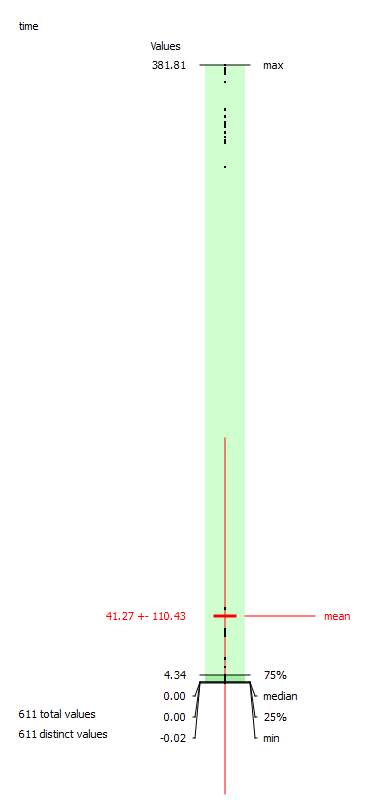
\includegraphics[width=0.6\linewidth]{2-Attribute-Statistics-time}}
    \caption{Компонент \texttt{2.\,Attribute~Statistics}. Статистические показатели свойства \texttt{time}.}
    \label{img:2-Attribute-Statistics-time}
\end{figure}

\begin{figure}[H]
    \center{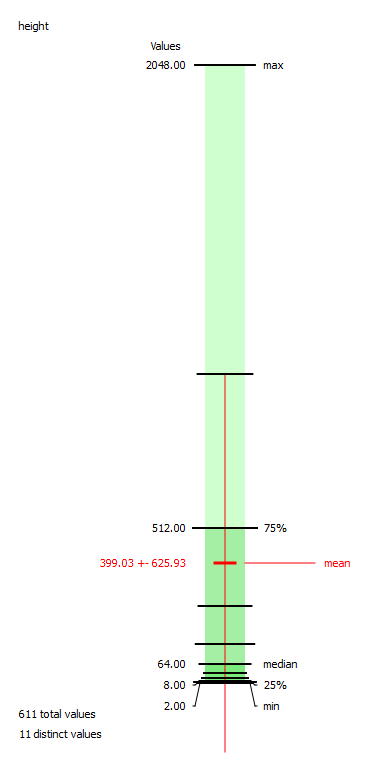
\includegraphics[width=0.6\linewidth]{2-Attribute-Statistics-height}}
    \caption{Компонент \texttt{2.\,Attribute~Statistics}. Статистические показатели свойства \texttt{height}.}
    \label{img:2-Attribute-Statistics-height}
\end{figure}

\begin{figure}[H]
    \center{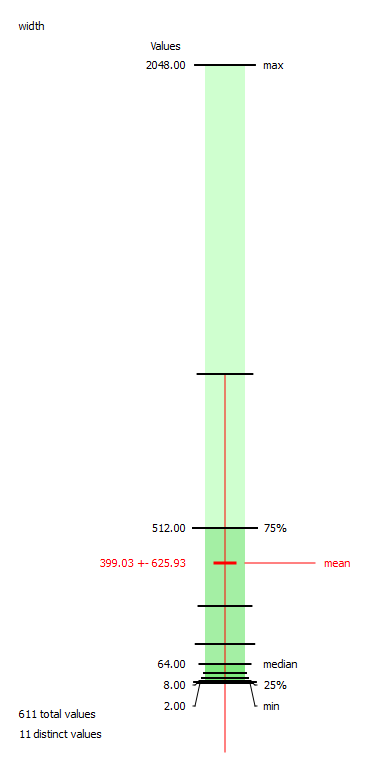
\includegraphics[width=0.6\linewidth]{2-Attribute-Statistics-width}}
    \caption{Компонент \texttt{2.\,Attribute~Statistics}. Статистические показатели свойства \texttt{width}.}
    \label{img:2-Attribute-Statistics-width}
\end{figure}

\begin{figure}[H]
    \center{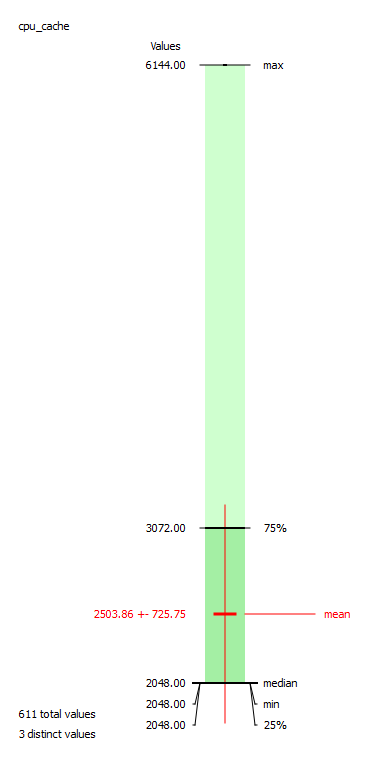
\includegraphics[width=0.6\linewidth]{2-Attribute-Statistics-cpu_cache}}
    \caption{Компонент \texttt{2.\,Attribute~Statistics}. Статистические показатели свойства \texttt{cpu_cache}.}
    \label{img:2-Attribute-Statistics-cpu_cache}
\end{figure}

\begin{figure}[H]
    \center{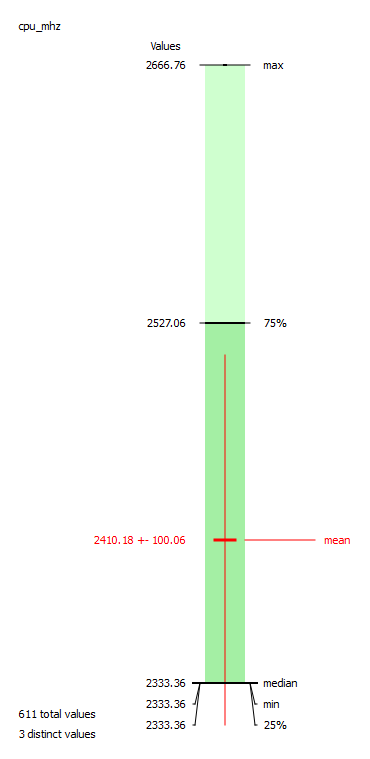
\includegraphics[width=0.6\linewidth]{2-Attribute-Statistics-cpu_mhz}}
    \caption{Компонент \texttt{2.\,Attribute~Statistics}. Статистические показатели свойства \texttt{cpu_mhz}.}
    \label{img:2-Attribute-Statistics-cpu_mhz}
\end{figure}

\begin{figure}[H]
    \center{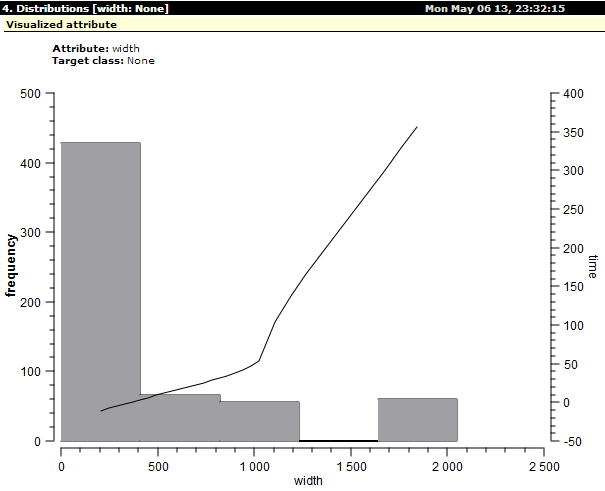
\includegraphics[width=0.7\linewidth]{4-Distributions-width}}
    \caption{Компонент \texttt{4.\,Distributions}. Распределение свойства \texttt{width} и его влияние на свойство \texttt{time}.}
    \label{img:4-Distributions-width}
\end{figure}

\begin{figure}[H]
    \center{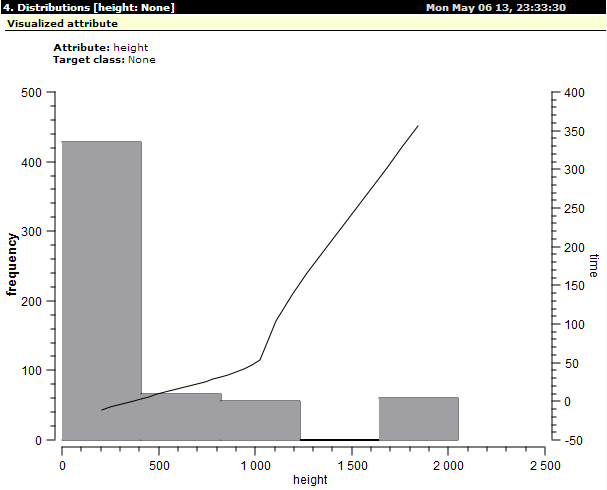
\includegraphics[width=0.7\linewidth]{4-Distributions-height}}
    \caption{Компонент \texttt{4.\,Distributions}. Распределение свойства \texttt{height} и его влияние на свойство \texttt{time}.}
    \label{img:4-Distributions-height}
\end{figure}

\begin{figure}[H]
    \center{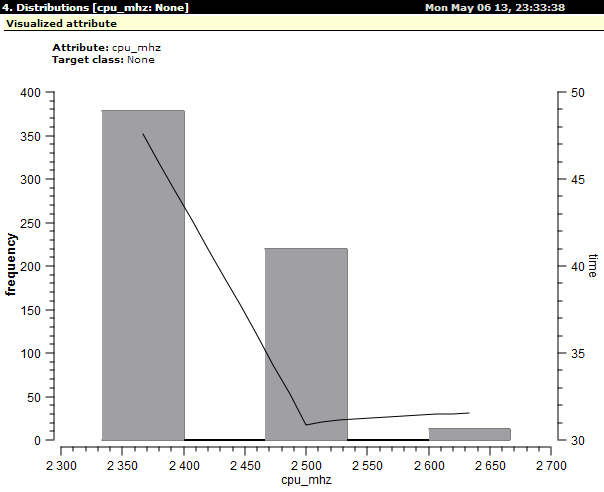
\includegraphics[width=0.7\linewidth]{4-Distributions-cpu_mhz}}
    \caption{Компонент \texttt{4.\,Distributions}. Распределение свойства \texttt{cpu_mhz} и его влияние на свойство \texttt{time}.}
    \label{img:4-Distributions-cpu_mhz}
\end{figure}

\begin{figure}[H]
    \center{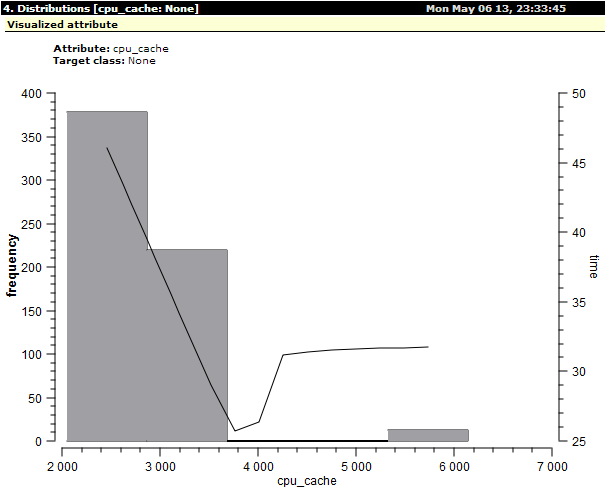
\includegraphics[width=0.7\linewidth]{4-Distributions-cpu_cache}}
    \caption{Компонент \texttt{4.\,Distributions}. Распределение свойства \texttt{cpu_cache} и его влияние на свойство \texttt{time}.}
    \label{img:4-Distributions-cpu_cache}
\end{figure}

\begin{figure}[H]
    \center{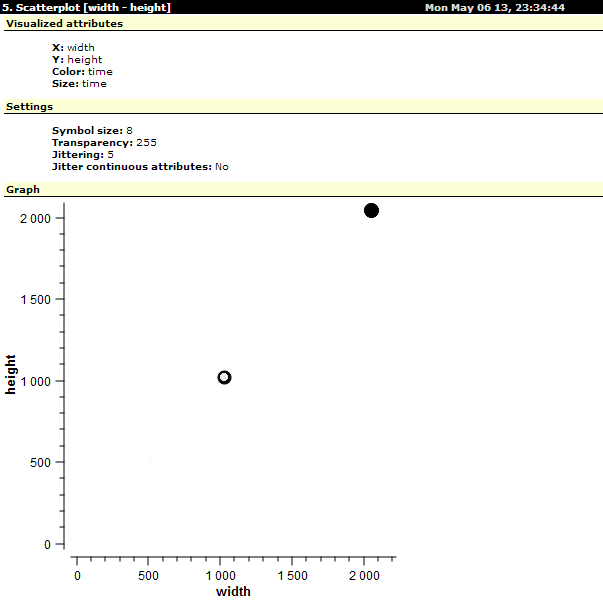
\includegraphics[width=0.7\linewidth]{5-Scatterplot}}
    \caption{Компонент \texttt{5.\,Scatterplot}. Зависимость свойства \texttt{time} от свойств \texttt{width} и \texttt{height}.}
    \label{img:5-Scatterplot}
\end{figure}
\end{document}
